% !TEX root = phy315book.tex




%----------------------------------------------------------------------------------------
%	PART 4 Chapters 35-42
%----------------------------------------------------------------------------------------

\part{Atomic Quantum States \label{part4}}

We finish with a series of models describing atomic systems and interactions between quantum systems.

\begin{figure}
\centering
\begin{tikzpicture}
\node[fill=blue!20,arrow box, text width=4.5cm, align=center, arrow box arrows={south:1cm},arrow box shaft width=1cm](p1) at (0,10) {\Large Quantum Angular Momentum};
\node[fill=blue!20,arrow box, text width=4.5cm, align=center, arrow box arrows={south:1cm},arrow box shaft width=1cm](p2) at (0,8) {\Large Hydrogen Atom Models};
\node[fill=blue!20,arrow box, text width=4.5cm, align=center, arrow box arrows={south:1cm},arrow box shaft width=1cm](p3) at (0,6) {\Large Numeric Quantum Models};
\node[fill=blue!20,rectangle, text width=4.5cm, align=center](p4) at (0,4) {\Large Quantum Beamsplitters};
\end{tikzpicture}
\end{figure}

%---------------------------------------
% Chapter 35
%---------------------------------------

\chapter{Angular Momentum Operators}

We return now to our three-dimensional quantum models. We now improve the model working in spherical coordinates that we started in Section \ref{sec:noncartesisanone}. We concentrate on potentials that are only dependent on the distance $r$ and not on the angular coordinates $\theta$ and $\phi$, $V(\vec{r}) = V(r)$. In this case, there are no external torques acting on the system and the angular momentum is conserved. That makes angular momentum a useful quantity to explore. We will first build a formalism for working with angular momentum, then we will use that to describe the wavefunctions of states in spherically symmetric quantum potentials.

\section{Angular Momentum Operator}
\begin{marginfigure}
\centering
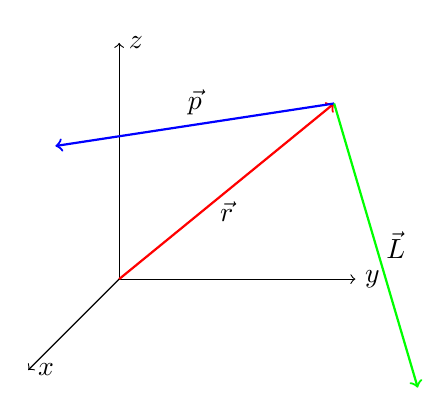
\begin{tikzpicture}
\draw[->](0,0,0) -- (3,0,0)node[right]{$y$};
\draw[->](0,0,0) -- (0,3,0)node[right]{$z$};
\draw[->](0,0,0) -- (0,0,3)node[right]{$x$};
\draw[->,red,thick](0,0,0) -- (3.5,3,2) node[midway,below,black]{$\vec{r}$};
\draw[->,blue,thick](3.5,3,2) -- (1.5,4,6)node[midway,above,black]{$\vec{p}$};
\draw[->,green,thick](3.5,3,2) -- (5.17,0,3.58) node[right,black,midway]{$\vec{L}$};
\end{tikzpicture}
\end{marginfigure}
The classical angular momentum vector is
\beq
\vec{L} = \vec{r}\times\vec{p} \rightarrow \begin{aligned}
L_x = & yp_z - zp_y\\
L_y = & zp_x - xp_z\\
L_z = & xp_y - yp_x.\\
\label{eq:ldefinition}
\end{aligned}
\eeq

As we've done before, we model the quantum angular momentum operator by turning the position and momentum into their corresponding quantum operators. That gives us the quantum angular momentum operator
\beq
\hat{\vec{L}} = \hat{\vec{R}} \times \hat{\vec{P}}\rightarrow \begin{aligned}
\hat{L}_x = & \hat{Y}\hat{P}_z - \hat{Z}\hat{P}_y\\
\hat{L}_y = & \hat{Z}\hat{P}_x - \hat{X}\hat{P}_z\\
\hat{L}_z = & \hat{X}\hat{P}_y - \hat{Y}\hat{P}_x.\\
\end{aligned}
\eeq
This is actually a set of three operators describing the three components of angular momentum. Any time we have multiple operators that act on a quantum state $\ket{\Psi}$, we need to know if they can be measured at the same time. To do this, we need to know the commutation relationships, Eq.~(\ref{XP commute}):\marginnote{\ref{tool:commutator}}% 
\beq
\begin{split}
\com{\hat{L}_x,\hat{L}_y} =& \I\hbar\hat{L}_z\\
\com{\hat{L}_y,\hat{L}_z} =& \I\hbar\hat{L}_x\\
\com{\hat{L}_z,\hat{L}_x} =& \I\hbar\hat{L}_y.
\label{eq:angmomcomm}
\end{split}
\eeq\arnote[-1cm]{Work these out using the commutation relationships for $\hat{X}$ and $\hat{P}_x$, and the other directions, too.}%
These are exactly the same relationships we found for the quantum spin model in Example \ref{ex:spincommutator}! 
\bas
\com{\hat{S}_x,\hat{S}_y} =& \I\hbar\hat{S}_z\\
\com{\hat{S}_y,\hat{S}_z} =& \I\hbar\hat{S}_x\\
\com{\hat{S}_z,\hat{S}_x} =& \I\hbar\hat{S}_y.
\eas
This relationship implies that there is a more general model we should build to which spin and angular momentum belong.

\section{General Angular Momentum}

We define the {\em general angular momentum} operators as any set of three Hermitian operators $\Jh_1$, $\Jh_2$, and $\Jh_3$ that satisfy the commutation relationships\marginnote{Typically we'll use the substitution $1\rightarrow x$, $2\rightarrow y$, and $3\rightarrow z$. Note that the indices are cyclic, staying in the order $123$, $231$, $312$. That is a special type of index ordering. If we flip any two indices in these, we pick up a $-1$.}%
\beq
\begin{split}
\com{\Jh_1,\Jh_2} =& \I\hbar\Jh_3\\
\com{\Jh_2,\Jh_3} =& \I\hbar\Jh_1\\
\com{\Jh_3,\Jh_1} =& \I\hbar\Jh_2.
\end{split}
\eeq
Although the individual components $\Jh_k$ do not commute with each other, they do commute with the operator associated with the dot product $\Ja^2\equiv \skew{4}\vec{\Ja}\cdot\skew{4}\vec{\Ja}$:
\beq
\Jh^2 = \Jh_1^2 + \Jh_2^2 +\Jh_3^2.
\eeq

\begin{exercise}
Show that
\beq
\com{\Jh^2,\Jh_1} = \com{\Jh^2,\Jh_2} = \com{\Jh^2,\Jh_3} = 0.
\label{eq:jsquarecomm}
\eeq

\end{exercise}
As we saw back in Section \ref{sec:eigenvadegen}, when we have multiple parameters that can describe a state that do not commute, we can still formulate a combined set of state vectors that do the best we can at describing the state. Because the individual angular momentum components $\Jh_k$ each commute with the $\Jh^2$, we could use any one of them, combined with the $\Jh^2$ operator to describe our angular momentum quantum state. Conventionally, we choose $\Jh_3$. This gives us a multi-parameter quantum state $\ket{j}\otimes\ket{m_j}\equiv\ket{jm_j}$ which is a joint eigenvector of these two operators. We now  need to find eigenvalues of these operators. 

The eigenvalues for these two combined states are
\bas
\Jh^2\ket{jm_j} = & j(j+1)\hbar^2\ket{jm_j}\\
\Jh_3\ket{jm_j} = & m_j\hbar\ket{jm_j}.
\eas\marginnote[-1.5cm]{The use of the term $j(j+1)$ in the eigenvalue for $\Jh^2$ will become clearer in a bit.}%
Because we've defined the general quantum state $\ket{\Psi} = \ket{jm_j}$, we can evaluate the expectation value of the operator $\Jh^2$ in this basis:
\beq
\bra{jm_j}\Jh^2\ket{jm_j} = \sum_k\bra{jm_j}\Jh_k^\dagger \Jh_k
\ket{jm_j} = \sum_k\avg{\psi_k|\psi_k} \geq 0
\eeq\marginnote[-1cm]{Because the $\Jh_k$ operators are Hermitian.}%
where $\ket{\psi_k} = \Jh_k\ket{jm_j}$. So the eigenvalues of $\Jh^2$ are positive or zero. This is similar to our situation with the number operator $\hat{N}$ for the quantum harmonic oscillator in Section \ref{sec:numberoperator}. In that section we found raising and lowering operators to step through the possible eigenstates. We do the same thing with our general angular momentum operators.

\section{Raising and Lowering Angular Momentum Operators}

We define the quantum angular momentum raising and lowering operators as
\beq
\Jpm = \Jh_1 \pm \I \Jh_2.
\eeq
We would like to re-write the $\Jh^2$ operator in terms of these raising and lowering operators, like we did with the number operator before. However, if we try $\Jp\Jm$, we get\arnote{Work out the expansion and use the general angular momentum operator definition.}%
\bas
\Jp\Jm =& \left(\Jh_1 + \I\Jh_2\right) \left(\Jh_1 - \I\Jh_2\right) \\
=& \Jh_1^2 + \Jh_2^2 -\I\com{\Jh_1,\Jh_2} \\
=& \Jh_1^2 + \Jh_2^2  + \hbar \Jh_3. \label{eq:jpjm}
\eas
%
\begin{exercise}
Show that
\beq
\Jm\Jp = \Jh_1^2 + \Jh_2^2  - \hbar \Jh_3.
\label{eq:jmjp}
\eeq
\end{exercise}

Putting these together, we can write the operator
\beq
\Jh^2 = \frac{1}{2}\left(\Jp\Jm + \Jm\Jp\right) + \Jh_3^2.
\eeq
With the total angular momentum operator written in this form, we can use the properties of the raising and lowering operators to find the eigenvalues of our eigenstate $\ket{jm_j}$.


\section{Properties of $\Jpm$}
Although $\Jpm$ commute with the total angular momentum operator
\beq
\com{\Jh^2,\Jpm} = \com{\Jh^2, \Jh_1 \pm \I\Jh_2} = 0,
\eeq
it does not commute with $\Jh_3$:
\bas
\com{\Jh_3,\Jpm} = & \com{\Jh_3, \Jh_1 \pm \I\Jh_2} \\
=& \com{\Jh_3,\Jh_1} \pm\I \com{\Jh_3,\Jh_2} \\
=& \pm\hbar \Jpm.
\eas\arnote[-1cm]{Fill in the missing steps.}
We now look at the overall effect of the $\Jh_3$ operator acting on a raised (or lowered) eigenstate:
\bas
\Jh_3\left(\Jpm\ket{jm_j}\right) = &\left(\Jpm \Jh_3 \pm \hbar \Jpm\right)\ket{jm_j}\\
=& \left(\Jpm m_j\hbar \pm \hbar \Jpm\right)\ket{jm_j} \\
=&\left( m_j \pm 1\right) \hbar \Jpm\ket{jm_j}.
\eas
So, as we saw with the raising and lowering operators for the quantum harmonic oscillator, the state $\Jpm\ket{jm_j}$ is an eigenstate of $\Jh_3$. We need to get the eigenvalues that include normalization for these new states. For now we'll start with
\beq
\Jpm \ket{jm_j} = c_\pm \hbar \ket{j(m_j\pm1)}
\eeq
where $c_\pm$ are the normalization constants we need to find. Since $\Jpm^\dagger = \Jh_\mp$, we evaluate the normalization for the raised (or lowered) state
\beq
1=\bra{jm_j}\Jh_\mp\Jpm\ket{jm_j} = \abs{c_\pm}^2\hbar^2
\label{eq:jpmnorm1}
\eeq
But we can also re-write Eqs.~ (\ref{eq:jpjm}) and (\ref{eq:jmjp}) as\arnote{Show this explicitly.}%
\bas
\Jm\Jp = & \Jh^2 - \Jh_3^2 + \hbar \Jh_3 \rmt{ and}\\ 
\Jp\Jm = &\Jh^2 - \Jh_3^2 - \hbar \Jh_3
\eas
so we evaluate the normalization condition to get the following two constants:
\bas
\bra{jm_j}\Jh_{+}\Jh_{-}\ket{jm_j} = & \bra{jm_j}\left(\Jh^2 - \Jh_3^2 + \hbar \Jh_3\right)\ket{jm_j} = \hbar^2\left[j(j+1) - m_j^2 + m_j\right]\\
\bra{jm_j}\Jh_{-}\Jh_{+}\ket{jm_j} = & \bra{jm_j}\left(\Jh^2 - \Jh_3^2 - \hbar \Jh_3\right)\ket{jm_j} = \hbar^2\left[j(j+1) - m_j^2 - m_j\right].
\eas
Combining these with Eq.~(\ref{eq:jpmnorm1}), we get the normalization constants
\beq
c_\pm = \sqrt{j(j+1) - m_j(m_j\pm1)}.
\eeq
So the raising and lowering operators, acting on the eigenstates of $\Jh^2$ and $\Jh_3$ give
\beq
\Jpm\ket{jm_j} = \hbar \sqrt{j(j+1) - m_j(m_j\pm1)} \ket{j(m_j\pm1)}.
\label{eq:jpmnormalized}
\eeq

Because the operator $\Jh_3$ is a component of the total angular momentum operator, we want the eigenvalues $m_j$ to be no bigger than the eigenvalues of $\Jh^2$:
\bas
\bra{jm_j}\Jh^2\ket{jm_j} = & \bra{jm_j}\Jh_1^2\ket{jm_j} +\bra{jm_j}\Jh_2^2\ket{jm_j} +\bra{jm_j}\Jh_3^2\ket{jm_j}\\
& \rmt{ so }j(j+1)\hbar^2 \geq m_j^2 \hbar^2\\
& \rmt{ or }m_j^2  \leq j(j+1).
\eas
This implies that there exists an $m_{j,\rmt{max}}$ and an $m_{j,\rmt{min}}$ so that
\beq
\Jp \ket{jm_{j,\rmt{max}}} = 0 \rmt{ and } \Jm \ket{jm_{j,\rmt{min}}} = 0.
\eeq
Using Eq.~(\ref{eq:jpmnormalized}), we get
\beq
\sqrt{j(j+1) - m_{j,\rmt{max}}(m_{j,\rmt{max}}+1)} = 0 \rmt{ which means }m_{j,\rmt{max}} = j.
\eeq
The same result applies for the other end: $m_{j,\rmt{min}} = -j$. Thus the values of $m_j$ range from
\beq
m_j = -j,-j+1,-j+2,\ldots,j-2,j-1,j.
\eeq
Because $\Jp$ steps $m_j$ through integer values ranging from $-j$ to $+j$, there are $2j$ total steps, which must be a non-negative integer. This means that 
\beq
j = 0,\frac{1}{2},1,\frac{3}{2},\ldots.
\eeq
The fact that the total angular momentum $j$ comes in both integer ($j=0,1,2,\ldots$) and half-integer ($j=1/2,3/2,5/2,\ldots$) steps is significant. The quantum systems with integer total spin are called {\em bosons} and behave differently in some models from systems with half-integer spin, called {\em fermions}. Putting all of this together, we have our model for working with general angular momentum:
\beq
\begin{split}
\Jh^2\ket{jm_j} = & j(j+1)\hbar^2\ket{jm_j}\\
\Jh_3\ket{jm_j} = & m_j\hbar \ket{jm_j} \\
j =& 0,\frac{1}{2},1,\frac{3}{2},\ldots \\ 
m_j =& -j,-j+1,-j+2,\ldots,j-2,j-1,j\; \rmt{ and}\\
\Jpm\ket{jm_j} = &\hbar \sqrt{j(j+1) - m_j(m_j\pm1)} \ket{j(m_j\pm1)}.
\label{eq:genangmom}
\end{split}
\eeq

\begin{exercise}
Show that the general angular momentum model, Eq.~(\ref{eq:genangmom}) works for the quantum spin states from Section \ref{sec:spinop} using the matrix representation where $j=1/2$ and $m_j = \pm1/2$.
\end{exercise}

\begin{exercise}
We focused most of our attention on $\Jh^{2}$ and $\Jh_{3}$, but what about $\Jh_{1}$ and $\Jh_{2}$?

\begin{enumerate}
\item[(a)] Show that
%
\bas
\Jh_{1} & =  \frac{1}{2}\left(\Jp + \Jm\right), \\
\Jh_{2} & =  -\frac{i}{2}\left(\Jh_{+} - \Jh_{-}\right).
\eas

\item[(b)] Use your result from the previous part to show that 
%
\bas
\Jh_{1}\ket{jm_j} = &  \frac{\hbar}{2}\left[\sqrt{j(j+1) - m_j(m_j + 1)}\ket{j(m_j+1)}\right.\\ 
& + \left.\sqrt{j(j+1) - m_j(m_j - 1)} \ket{j(m_j-1)}    \right], \\
\Jh_{2}\ket{jm_j} = & -\frac{\I\hbar}{2}\left[\sqrt{j(j+1) - m_j(m_j + 1)}\ket{j(m_j+1)}\right. \\
& -\left. \sqrt{j(j+1) - m_j(m_j - 1)} \ket{j(m_j-1)}  \right].
\eas


\item[(c)] Show that the average value of $\Jh_{1}$ and $\Jh_{2}$ for a quantum system in the angular momentum state $\ket{jm_j}$ vanishes:
%
\beq
\bra{jm_j}\Jh_{1}\ket{jm_j} = \bra{jm_j}\Jh_{2}\ket{jm_j} = 0.
\eeq


\item[(d)] Show that the average value of $\Jh_{1}^{2}$ and $\Jh_{2}^{2}$ for a quantum system in the angular momentum state $\ket{jm_j}$ is given by:
%
\begin{equation}
\bra{jm_j}\Jh_{1}^2\ket{jm_j} = \bra{jm_j}\Jh_{2}^2\ket{jm_j} = \frac{\hbar^{2}}{2}\left[j(j+1) - m_j^{2}\right].
\end{equation}

\end{enumerate}
\end{exercise}

%---------------------------------------


%---------------------------------------
% Chapter 36
%---------------------------------------

\chapter{Orbital and Spin Angular Momentum}

We now model orbital angular momentum and then connect it to spin angular momentum that we used previously. We modeled the total angular momentum operator and the $z$-component of the angular momentum with their eigenvalues and eigenvectors as
\beq
\begin{split}
\hat{L}^2\ket{lm_l} =& l(l+1)\hbar^2\ket{lm_l} \\
\hat{L}_z\ket{lm_l} = & m_l\hbar\ket{lm_l}
\end{split}
\label{eq:oameigenvalue}
\eeq
where $l$ is the total angular momentum quantum number and $m_l$ is the $z$-component quantum number. \marginnote[-2cm]{Recall that we only need two real numbers to specify a direction in 3-vector space. These two numbers are all we need to fully parametrize the angular momentum quantum state.} These joint eigenvectors are orthonormal, $\avg{lm_l|l'm_l'} = \delta_{ll'}\delta_{m_lm_l'}$. 


\begin{exercise}
The rigid rotator can be used to model a diatomic molecule.  Consider a rotator consisting of two atoms of mass $m$ joined by a massless rigid bar of length $a$.  It is free to spin about any axis passing through its center, but the center is fixed in space.

\begin{enumerate}
\item[(a)]  Write down the classical Hamiltonian for this system.  Express it in terms of its angular momentum $L$ and moment of inertia $I$.

\item[(b)] Find the moment of inertia appropriate for this system.

\item[(c)]  Now quantize this system, and show that the energies of the quantum rigid rotator are
%
\begin{equation}
E_{n} = \frac{\hbar^{2}n(n + 1)}{ma^{2}}, \,\,\,\,\, n = 0, 1, 2, \ldots.
\end{equation}
%
\item[(d)]  Find the energy spacing between adjoining energy levels, $E_{n+1} - E_{n}$.

\item[(e)]  Plug in some numbers.  Assume the particles are hydrogen atoms and $a \sim 1$~\AA.  Find the energy spacing between the lowest two energy levels.  Express your answer in eV.

\end{enumerate}
\end{exercise}


\section{Orbital Angular Momentum in the Position Basis}
We want to model our angular momentum eigenstates in the position basis so we can use them to describe quantum systems with radially-symmetric potentials and non-zero angular momentum. As we did in Section \ref{sec:momentuminposbasis}, we write the momentum operator in the position basis. However, working in three-dimensions means that the three-dimensional momentum operator in the position basis is
\beq
\bra{\vec{r}}\hat{\vec{P}}\ket{\vec{r}\,'} = -\I\hbar\delta(\vec{r}-\vec{r}\,')\vec{\nabla}\,'
\eeq\marginnote[-1cm]{In Cartesian coordinates\beq\vec{\nabla}=\hat{x}\frac{\partial}{\partial x}+\hat{y}\frac{\partial}{\partial y}+\hat{z}\frac{\partial}{\partial z}.\eeq}%
where the gradient $\vec{\nabla}$ is the three-dimensional version of the derivative operator. However, because we are interested in spherically symmetric potentials, it makes sense to work in spherical coordinates where
\beq
\vec{\nabla} = \hat{r}\frac{\partial}{\partial r} + \hat{\theta}\frac{1}{r}\frac{\partial}{\partial\theta} + \hat{\phi}\frac{1}{r\sin\theta}\frac{\partial}{\partial\phi}.
\eeq%
\begin{marginfigure}
\centering
\begin{tikzpicture}[scale=1.3]
\draw[->](0,0,0) -- (3,0,0)node[right]{$y$};
\draw[->](0,0,0) -- (0,3,0)node[right]{$z$};
\draw[->](0,0,0) -- (0,0,3)node[right]{$x$};
\draw[->,thick](0,0,0) -- (1.5,1,0.8)node[above,midway]{$r$};
\draw[dashed] (0,0,0) -- (1.5,0,.8);
\begin{scope}[rotate around={30:(0,0)}]
    \draw (0:0.5) arc (0:62:0.5)node[midway,above]{$\theta$};
\end{scope}

\begin{scope}[canvas is xz plane at y=0, rotate around={90:(0,0)}]
    \draw (0:0.5) arc (0:-62:0.5)node[midway,below]{$\phi$};
\end{scope}

\draw[dashed] (1.5,1,0.8) -- (1.5,0,.8);
\draw[dashed] (0,0,.8) -- (1.5,0,.8);
\draw[dashed] (1.5,0,0) -- (1.5,0,.8);
\draw[dashed](1.5,1,.8) -- (2,1.33,1.1);
\draw[->,thick,red](2,1.33,1.1) -- (2.8,1.86,1.5)node[right,black]{$\hat{r}$};
\draw[->,thick,green](2,1.33,1.1) -- (2.5,0.47,1.33)node[right,black]{$\hat{\theta}$};
\draw[->,thick,blue](2,1.33,1.1) -- (2.1,1.8,0.22)node[right,black]{$\hat{\phi}$};
\draw[dotted,->](2,1.33,1.1) -- (3,1.33,1.1);
\draw[dotted,->](2,1.33,1.1) -- (2,2.33,1.1);
\draw[dotted,->](2,1.33,1.1) -- (2,1.33,2.1);
\end{tikzpicture}
\end{marginfigure}%
We now need to express $\vec{L} = \vec{r}\times\vec{p}$ in spherical coordinates. Because $\vec{r} = r\hat{r}$, the angular momentum operator  in the position basis, is
\beq
\bra{\vec{r}}\hat{\vec{L}}\ket{\vec{r}\,'} = -\I\hbar\delta(\vec{r} - \vec{r}\,')\left[r'(\hat{r}'\times\hat{r}')\frac{\partial}{\partial r'} + (\hat{r}'\times\hat{\theta}')\frac{\partial}{\partial\theta'} + (\hat{r}'\times\hat{\phi}')\frac{1}{\sin\theta'}\frac{\partial}{\partial\phi'}  \right].
\eeq
We evaluate the cross products of the unit vectors: $(\hat{r}'\times\hat{r}')=0$, $(\hat{r}'\times\hat{\theta}') = \hat{\phi}'$, and $(\hat{r}'\times\hat{\phi}') = -\hat{\theta}'$. That means that the angular momentum vector is
\beq
\bra{\vec{r}}\hat{\vec{L}}\ket{\vec{r}\,'}= -\I\hbar\delta(\vec{r} - \vec{r}\,')\left[\hat{\phi'}\frac{\partial}{\partial\theta'} -\hat{\theta}'\frac{1}{\sin\theta'}\frac{\partial}{\partial\phi'}  \right]
\label{eq:linposbasis}
\eeq
and
\beq
\bra{\vec{r}}\hat{L}^2\ket{\vec{r}\,'}= -\hbar^2\delta(\vec{r} - \vec{r}\,')\left[\frac{1}{\sin\theta'}\frac{\partial}{\partial\theta'}\left(\sin\theta'\frac{\partial}{\partial \theta'}\right) + \frac{1}{\sin^2\theta'}\frac{\partial}{\partial\phi'^2} \right].
\label{eq:lsquaredinposbasis}
\eeq

\begin{exercise}
Show that Eq.~(\ref{eq:lsquaredinposbasis}) comes from Eq.~(\ref{eq:linposbasis}). Use the dot product in polar coordinates:
\beq
\vec{U}\cdot\vec{V} = U_rV_r  + U_\theta V_\theta + U_\phi V_\phi
\eeq
and the derivatives of the unit vectors:
\bas
\frac{\partial \hat{\phi}}{\partial\theta} &= 0 & \frac{\partial \hat{\theta}}{\partial\theta} &= -\hat{r}\\
\frac{\partial \hat{\phi}}{\partial\phi} &= -\cos\theta\hat{\theta}-\sin\theta\hat{r} & \frac{\partial \hat{\theta}}{\partial\phi} &= \cos\theta\hat{\phi}.
\eas

\end{exercise}

We also need the $z$-component of the angular momentum in spherical coordinates. The only vector component of $\vec{L}$ along the $z$-direction is from $\hat{\theta}_z = -\sin\theta$. This means that
\beq
\bra{\vec{r}}\hat{L}_z\ket{\vec{r}\,'}= -\I\hbar\delta(\vec{r} - \vec{r}\,')\frac{\partial}{\partial\phi'}.
\label{eq:lzinposbasis}
\eeq
We now have everything we need to find the orbital angular momentum wavefunctions in the position basis.

\section{Orbital Angular Momentum Wavefunction}

We project the position basis $\bra{\vec{r}}$ on to the eigenvalue relationships, Eq.~(\ref{eq:oameigenvalue}):
\beq
\begin{split}
\bra{\vec{r}}\hat{L}^2\ket{lm_l} =& l(l+1)\hbar^2\avg{\vec{r}|lm_l} \\
\bra{\vec{r}}\hat{L}_z\ket{lm_l} = & m_l\hbar\avg{\vec{r}|lm_l}
\end{split}
\eeq
We now insert the completeness relationship on the left and project out of the integrals using the Dirac delta function. This gives us the two differential equations
\beq
\begin{split}
-\hbar^2\left[\frac{1}{\sin\theta}\frac{\partial}{\partial\theta}\left(\sin\theta\frac{\partial}{\partial \theta}\right) + \frac{1}{\sin^2\theta}\frac{\partial}{\partial\phi^2} \right] \Ylm(\theta,\phi)=& l(l+1)\hbar^2 \Ylm(\theta,\phi) \\
-\I\hbar\frac{\partial}{\partial\phi}\Ylm(\theta,\phi) = & m_l\hbar \Ylm(\theta,\phi)
\end{split}
\eeq\arnote[-2cm]{I skipped steps here. Make sure you write them out in your notes.}%
where we've defined the angular wavefunction $\avg{\vec{r}|lm_l}\equiv \Ylm(\theta,\phi)$.\marginnote{This ignores the radial components. For now, this simplified model will work, but we will have to treat those later.} These are two differential equations that have known solutions. We'll start with the second equation.

\subsection{The $\phi$-dependence of $\Ylm$}
The $z$-direction differential equation, simplified, is
\beq
\frac{\partial}{\partial\phi}\Ylm(\theta,\phi) =  \I m_l \Ylm(\theta,\phi).
\eeq
This has solutions
\beq
\Ylm(\theta,\phi) = \Ylm(\theta,0)\E{\I m_l\phi}
\label{eq:ylmphi}
\eeq
where $\Ylm(\theta,0)$ is the angular wavefunction at $\phi=0$, determined by the initial conditions of the state. Our boundary conditions also require that, because the wavefunction must be continuous, we have%
\beq
\Ylm(\theta,\phi) = \Ylm(\theta,\phi+2\pi).
\eeq%
\begin{marginfigure}
\centering
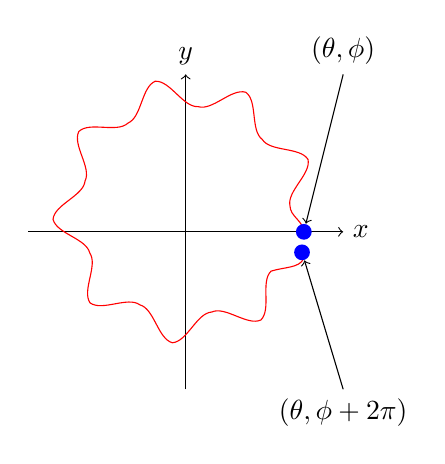
\begin{tikzpicture}
\draw[->](-2,0) -- (2,0)node[right]{$x$};
\draw[->](0,-2) -- (0,2)node[above]{$y$};
\draw[red,->,decorate, decoration={snake,amplitude=5,segment length=30, post length=.05cm}](1.5,0)node[fill=blue,circle, minimum size=0.2cm,inner sep=0pt](A){} arc (0:350:1.5)node[fill=blue,circle, minimum size=0.2cm,inner sep=0pt](B){};
\draw[->] (2,2) node[above]{$\Ylm(\theta,\phi)$} -- (A);
\draw[->] (2,-2) node[below]{$\Ylm(\theta,\phi+2\pi)$} -- (B);
\end{tikzpicture}
\end{marginfigure}%
This means that 
\beq
\E{\I m_l \phi} = \E{\I m_l \phi}\E{\I m_l 2\pi},
\eeq
so $m_l$ must be an integer. We also know from our general angular momentum discussion that $m_l$ ranges from $-l$ to $l$, so that implies that $l$ must also be an integer. We therefore have
\beq
\begin{split}
m_l =& -l,-l+1,-l+2,\ldots l-2,l-1,l\;\; \rmt{ and }\\
l=& 0,1,2,3,\ldots.
\end{split}
\eeq


\subsection{The $\theta$-dependence of $\Ylm$}
We now solve the other differential equation:
\beq
\left[\frac{1}{\sin\theta}\frac{\partial}{\partial\theta}\left(\sin\theta\frac{\partial}{\partial \theta}\right) + \frac{1}{\sin^2\theta}\frac{\partial}{\partial\phi^2} \right] \Ylm(\theta,\phi)= -l(l+1) \Ylm(\theta,\phi) 
\eeq
knowing that the $\phi$ dependence is given by Eq.~(\ref{eq:ylmphi}), we can simplify this further to
\beq
\frac{1}{\sin\theta}\frac{\partial}{\partial\theta}\left(\sin\theta\frac{\partial}{\partial \theta}\right)\Ylm(\theta,0) - \frac{m_l^2}{\sin^2\theta}\Ylm(\theta,0) = -l(l+1) \Ylm(\theta,0).
\eeq\arnote[-1.5cm]{Again, I've skipped steps. Plug in the solution from the $\phi$ dependence, take the derivatives, and cancel the exponentials.}%
This differential equation has two solutions consisting of the Legendre $P$ and $Q$ polynomials,
\beq
\Ylm(\theta,0) = A P_l^{m_l}(\cos\theta) + B Q_l^{m_l}(\cos\theta)
\eeq
However, the Legendre $Q$ polynomials do not converge, so our boundary conditions imply that the constant $B=0$. We need to normalize the total wavefunction
\beq
\Ylm(\theta,\phi) = A P_l^{m_l}(\cos\theta) \E{\I m_l\phi}.
\eeq
The normalization integral is 
\beq
\avg{lm_l|lm_l} = \int\displaylimits_{0}^{2\pi}d\phi\int\displaylimits_{0}^{\pi}d\theta \sin\theta {\Ylm}^*(\theta,\phi)\Ylm(\theta,\phi) = 4\pi \frac{(l+m_l)!}{(2l+1)(l-m_l)!}\abs{A}^2
\eeq\marginnote{Other texts use the convention that there is an extra negative factor $(-1)^{m_l}$ out front if $m_l<0$. However, modern \CAS's can handle the negative numbers just fine without it.}%
which means that 
\beq
A = \sqrt{\frac{(2l+1)(l-m_l)!}{4\pi(l+m_l)!}}.
\eeq
So that means that the wavefunctions, called the {\em spherical harmonics} are
\beq
\Ylm(\theta,\phi)=\sqrt{\frac{(2l+1)(l-m_l)!}{4\pi(l+m_l)!}} P_l^{m_l}(\cos\theta) \E{\I m_l\phi}.
\eeq
The first handful of spherical harmonics are shown in Table \ref{table:sphar}.

\begin{table*}

\begin{tabular}{|c|c|c|c|}
\hline
& $m_l=0$ &  $m_l=\pm1$ &  $m_l=\pm2$ \\
\hline
&&&\\
$l=0$& $\displaystyle Y_0^0 = \sqrt{\frac{1}{4\pi}}$&   &   \\
&&&\\
$l=1$& $\displaystyle  Y_1^0 = \sqrt{\frac{3}{4\pi}}\cos\theta$ & $ \displaystyle  Y_1^{\pm1} = \mp\sqrt{\frac{3}{8\pi}}\sin\theta\E{\pm\I\phi}$   &   \\
&&&\\
$l=2$& $\displaystyle  Y_2^0 = \sqrt{\frac{5}{16\pi}}(3\cos^2\theta-1)$ & $ \displaystyle  Y_2^{\pm1} = \mp\sqrt{\frac{15}{8\pi}}\sin\theta\cos\theta\E{\pm\I\phi}$   &  $ \displaystyle  Y_2^{\pm2} = \sqrt{\frac{15}{32\pi}}\sin^2\theta\E{\pm\I 2\phi}$  \\
&&&\\
\hline
\end{tabular}
\caption[][1cm]{The first handful of spherical harmonics.}
\label{table:sphar}
\end{table*}

The spherical harmonics are a complete orthornormal set. We can therefore write any function $f(\theta,\phi)$ on the surface of a sphere in terms of a sum of the spherical harmonics,
\beq
f(\theta,\phi) = \sum_{l=0}^\infty\sum_{m_l=-l}^{l}c_{l,m_l}\Ylm(\theta,\phi)
\eeq
where the coefficients $c_{l,m_l}$ are constants.


\begin{exercise}
Using the spherical harmonics in Table \ref{table:sphar}, show that the spherical harmonics are orthonormal:
\beq
\avg{lm_l|l'm_l'} = \int\displaylimits_{0}^{2\pi}d\phi\int\displaylimits_{0}^{\pi}d\theta \sin\theta \left[{\Ylm}(\theta,\phi)\right]^{*}Y_{l'}^{m_l'}(\theta,\phi) = \delta_{ll'}\delta_{m_lm_l'}.
\eeq
\end{exercise}

\section{Combined Spin and Angular Momentum}

Although the quantum numbers $l$ are only allowed to be integers in order to model orbital angular momentum, we found previously that the $j$ quantum numbers could also be half-integers. We found that our quantum spin model had a half-integer value of $s=1/2$. When we combine both orbital angular momentum and spin angular momentum, we use the broader range of possible $j$ values.

Our models for spin and orbital angular momentum both described these using 3-vectors: $\vec{S}$ and $\vec{L}$. The combination of these is also a vector, which is typically called the {\em total angular momentum} vector operator is denoted as%
\begin{marginfigure}
\centering
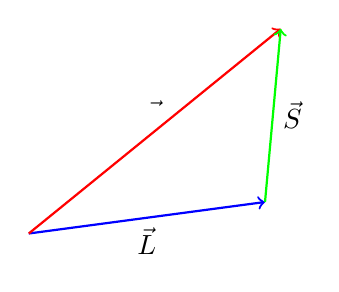
\begin{tikzpicture}
\draw[->,blue,thick] (0,0) -- (3,.4)node[below,midway,black]{$\vec{L}$};
\draw[->,red,thick] (0,0) -- (3.2,2.6)node[above,midway,black]{$\vec{\Ja}$};
\draw[->,green,thick] (3,.4) -- (3.2,2.6)node[right,midway,black]{$\vec{S}$};
\end{tikzpicture}
\end{marginfigure}%
\beq
\skew{4}\hat{\skew{4}\vec{\Ja}} = \hat{\vec{L}} + \hat{\vec{S}}.
\label{eq:combinedangspin}
\eeq
The total angular momentum quantum number ranges from $j_\rmt{max} = l + s$ to the value $j_\rmt{min} = \abs{l-s}$.\marginnote{Roughly, this comes from the point where the spin is aligned with the angular momentum and when it is anti-aligned. A more rigorous proof can be found elsewhere.} The $z$-component quantum number $m_j$ ranges from $-j$ to $+j$ as we've seen previously. We choose which model to use depending on the situation. We'll see later when we look at spin-orbit coupling in the hydrogen atom that the best model to use is this combined total angular momentum model.

We can also combine spin angular momentum vectors. We model the combined effect of both an electron with spin $s=1/2$ and a nucleus consisting of a single proton which also has spin-$1/2$. However, to distinguish the nuclear spin from the electron spin, we denote the nuclear spin as $\vec{I}$.\marginnote{This notation is used in atomic physics contexts more than in nuclear physics contexts.} We thus have a product state of the electron and nuclear spin. We will work in a common $z$-basis for both spins. The product state, following our model from Chapter \ref{ch:mqs}, is 
\beq
\ket{\Psi} = \underbrace{\left(\alpha_u\ket{u} + \alpha_d\ket{d}\right)}_{\displaystyle \vec{S}\rmt{ electron}} \otimes \underbrace{\left(\beta_u\ket{u} + \beta_d\ket{d}\right)}_{\displaystyle \vec{I}\rmt{ nucleus}}.
\eeq
There are four possible product states in this model and the total state is written as the arbitrary sum of all four:
\beq
\ket{\Psi} = \alpha_u\beta_u\ket{uu} + \alpha_u\beta_d\ket{ud} + \alpha_d\beta_u\ket{du} + \alpha_d\beta_d\ket{dd}.
\label{eq:prodstatespinSI}
\eeq
There are times, however, where it is better to work in a combined spin basis instead of the separate product state bases. We define the total spin operator of this system as\marginnote{Again this notation is used in atomic physics.}%
\beq
\hat{\vec{F}} \equiv \hat{\vec{S}} + \hat{\vec{I}}
\label{eq:nucleartotalspin}
\eeq
and define the eigenstates as $\ket{fm_f}$. In this basis we have the same pattern as our general angular momentum model where
\bas
\hat{F}^2\ket{fm_f} = & f(f+1)\hbar^2\ket{fm_f}\\
\hat{F}_z \ket{fm_f} = & m_f\hbar\ket{fm_f}.
\eas
We will revisit this model when build a model for describing the spin-spin coupling in hydrogen.


\begin{exercise}

The {\em singlet } state we saw in Chapter \ref{ch:mqs} can be written in terms of the $\ket{fm_f}$ basis as
\beq
\ket{00} = \frac{1}{\stwo}\left(\ket{ud} - \ket{du}\right).
\eeq
We now find the $\ket{fm_f}=\ket{1\;1}$ and $\ket{1\;{-1}}$ states when given the triplet state  $\ket{fm_f}=\ket{1\;1}=\ket{uu} $ .  We start by defining the total spin ladder operators
%
\beq
\hat{F}_{\pm} \equiv \hat{S}_{\pm} + \hat{I}_{\pm},
\eeq
%
where $\hat{S}_{\pm}$ and $\hat{I}_{\pm}$ are the ladder operators for the electron and nuclear spins:
\beq
\hat{S}_{\pm}\ket{sm_{s}}=  \sqrt{s(s+1) - m_{s}(m_{s} \pm 1)}\,\hbar\ket{s(m_{s}\pm1)}.
\eeq
Apply $\hat{F}_{-}$ twice to $\ket{11}$ and show that the results are given by 
%
\bas
\ket{fm_f} = \ket{1\;0} & =  \frac{1}{\sqrt{2}}\left(\ket{ud}+\ket{du}\right), \\
\ket{1\;{-1}} & = \ket{dd}.
\eas
%

\end{exercise}


%---------------------------------------
\chapter{Radially Symmetric Potentials}

We are now ready to add a radially symmetric potential $V(\vec{r}) = V(r)$ to our model. We model the Hamiltonian operator as
\beq
\hat{H} = \frac{\hat{P}^2}{2m} + V(\hat{R})
\eeq
with the Schr\"{o}dinger equation\marginnote{\ref{tool:sch}}%
\beq
\I\hbar\frac{\partial\ket{\Psi}}{\partial t} = \hat{H}\ket{\Psi} = E\ket{\Psi}.
\eeq
We project this onto the position basis in spherical coordinates and get the TISWE\marginnote{\ref{tool:TISWE}}%
\beq
-\frac{\hbar^2}{2m}\nabla^2\psi_E(\vec{r}) + V(r)\psi_E(\vec{r}) = E \psi_E(\vec{r})
\eeq
where the differential operator is\marginnote{This is known as {\em conservation of messiness} where the potential is written as a simple function of $r$, but the gradient is messy.}%
\beq
\nabla^2 = \frac{1}{r^2}\frac{\partial}{\partial r}\left(r^2\frac{\partial}{\partial r}\right) + \frac{1}{r^2}\left[ \frac{1}{\sin\theta}\frac{\partial}{\partial\theta}\left(\sin\theta\frac{\partial}{\partial\theta}\right) + \frac{1}{\sin^2\theta}\frac{\partial^2}{\partial\phi^2}\right].
\eeq
However, we've already seen part of this: the piece in the square brackets is just the total angular momentum operator in the position basis, 
\beq
-\frac{\bra{\vec{r}}\hat{L}^2\ket{\vec{r}\,'}}{\hbar^2\delta(\vec{r}-\vec{r}\,')}.
\eeq
So we define a new {\em radial momentum} operator $\hat{P}_r^2$ such that\marginnote{This radial momentum ``operator'' doesn't really behave like quantum mechanical momentum operators. We need to consider the entire momentum for that to work. However, it is a useful short-hand for the derivatives and helps clean up the calculations. We are also treating the $1/r^2$ term like it is a constant, not an operator.}% 
\beq
\bra{\vec{r}}\hat{P}_r^2\ket{\vec{r}\,'} = -\hbar^2 \delta(\vec{r}-\vec{r}\,') \frac{1}{r'^2}\frac{\partial}{\partial r'}\left(r'^2\frac{\partial}{\partial r'}\right).
\eeq
The Hamiltonian operator in the position basis is thus
\beq
\hat{H} = \frac{1}{2m} \left(\hat{P}_r^2 + \frac{1}{r^2}\hat{L}^2\right) + V(\hat{R}).
\eeq
So the eigenvectors of our Hamiltonian for radially symmetric potentials must be a product state of the angular momentum eigenvectors and a radial eigenvector,
\beq
\ket{\psi_E} = \ket{\psi_r}\otimes\ket{lm_l}.
\eeq
The time-independent Schr\"{o}dinger equation is then
\bas
\hat{H}\ket{\psi_E} = & \left[\frac{1}{2m} \left(\hat{P}_r^2 + \frac{1}{r^2}\hat{L}^2\right) + V(\hat{R})\right]\left(\ket{\psi_r}\otimes\ket{lm_l}\right)\\
=&\left(\frac{1}{2m}\hat{P}_r^2\ket{\psi_r} + V(\hat{R})\ket{\psi_r}\right)\otimes\ket{lm_l} + \ket{\psi_r}\otimes\left(\frac{1}{2mr^2}\hat{L}^2\ket{lm_l}\right)\\
=&\left(\frac{1}{2m}\hat{P}_r^2\ket{\psi_r} + V(\hat{R})\ket{\psi_r}\right)\otimes\ket{lm_l} + \frac{\hbar^2 l(l+1)}{2mr^2}\ket{\psi_r}\otimes\ket{lm_l}
\eas
where we used the eigenvalue equation for $\hat{L}^2$ in the last step. We now factor out the common $\ket{lm_l}$ term to get
\beq
\left(\frac{1}{2m}\hat{P}_r^2 + V(\hat{R}) + \frac{\hbar^2 l(l+1)}{2mr^2}\right)\ket{\psi_r}\otimes\ket{lm_l} = E \ket{\psi_r}\otimes\ket{lm_l}.
\eeq
We project both sides with $\bra{lm_l}$ and get an operator equation for the radial state only:
\beq
\left(\frac{1}{2m}\hat{P}_r^2 + V(\hat{R}) + \frac{\hbar^2 l(l+1)}{2mr^2}\right)\ket{\psi_r} = E \ket{\psi_r}.
\eeq
We now project this onto the position basis and define the radial wavefunction $R(r)\equiv \avg{\vec{r}|\psi_r}$.\marginnote{Our complete model is now $\avg{\vec{r}|\Psi}=\avg{\vec{r}|\psi_r(lm_l)} = R(r)\Ylm(\theta,\phi)$} The TISWE for the radial wavefunction is then
\beq
\frac{-\hbar^2}{2m r^2}\frac{\partial}{\partial r}\left(r^2\frac{\partial R(r)}{\partial r}\right) + V(r)R(r) + \frac{\hbar^2 l(l+1)}{2mr^2}R(r) = E R(r).
\label{eq:radialTISWE}
\eeq\arnote[-0.5cm]{I've skipped a couple of steps here. Fill them out in your notes.}%

\section{Spherical Quantum Dot}
We are now ready to improve our model of a spherical quantum dot that we first used in Example \ref{ex:sphericalpotential1}. We model the quantum dot as having a constant (zero) potential inside a radius $a$ and infinite outside that radius:
\beq
V(r) = \begin{cases}0 & r\leq a\\ \infty &\abs{r} >a. \end{cases}
\eeq
We now solve the radial wave equation, Eq.~(\ref{eq:radialTISWE}) for $V(r)=0$, noting that it is helpful to define the wave number
\beq
k^2 = \frac{2 m E}{\hbar^2}.
\eeq
The solutions are spherical Bessel functions $j_n(x)$ and $y_n(x)$:
\beq
R(r) = A j_{l}\left(k r\right) + B y_{l}\left(k r\right).
\eeq
The $y_n(x)$ functions go to infinity at $r=0$, so the constant $B=0$ so our solutions are normalizable. Finally we want $R(a) = 0$ so we look for zeros of the spherical Bessel functions that work such that $j_l(ka)=0$. As with the one-dimensional infinite quantum well model, this leads to quantized energies in order to satisfy the boundary condition. The total wavefunction needs to be normalized as well.
\begin{exercise}
Calculate the first four energy levels for an electron confined to an spherical quantum dot with radius $a\approx6$~nm. Normalize these radial wavefunctions and plot them.\marginnote{Recall that the normalization integral is $\int_0^a r^2 j_l(kr)j_l(kr)dr$.}
\end{exercise}

\section{Coulomb Potential Well}
A simple model of the interaction between an electron (mass $m$) and a proton (both with charge $e$) in a hydrogen atom describes their interaction potential as
\begin{marginfigure}[1cm]
\centering
\begin{tikzpicture}
\draw[->] (0,0) -- (4,0) node[right]{$r$};
\draw[->] (0,-3) -- (0,1) node[above]{$V(r)$};
\begin{scope}
\clip (0,-3) rectangle (4,1);
\draw[domain=0.2:4,samples=100,red] plot({\x},{-1/(\x)});
\end{scope}
\draw[blue,thick,dashed](0,-1) -- (1,-1)node[right,black]{$E$};
\end{tikzpicture}
\end{marginfigure}
\beq
V(r) = -\frac{1}{4\pi\epsilon_0}\frac{e^2}{r}.
\eeq
We are modeling the proton as having infinite mass so that it doesn't move. We are also modeling both the electron and the proton as not having any quantum spin. We model the electron as a quantum system that follows our MWM. The radial wave equation (Eq.~(\ref{eq:radialTISWE})) is then
\beq
\frac{-\hbar^2}{2m r^2}\frac{\partial}{\partial r}\left(r^2\frac{\partial R(r)}{\partial r}\right) - \frac{e^2}{4\pi\epsilon_0}\frac{R(r)}{r} + \frac{\hbar^2 l(l+1)}{2mr^2}R(r) = E R(r).
\label{eq:radialhamiltonian}
\eeq
We likewise define the wave number as before: $k^2 = -2mE/\hbar^2$, noting that $E<0$ for bound states so $k^2>0$. The radial wave equation is thus
\beq
\frac{1}{r^2}\frac{\partial}{\partial r}\left(r^2\frac{\partial R(r)}{\partial r}\right) + \frac{2me^2}{4\pi\epsilon_0\hbar^2}\frac{R(r)}{r} - \frac{l(l+1)}{r^2}R(r) = k^2 R(r).
\eeq
The solutions to the wave equation are a hypergeometric $U_a^b(z)$ function and a Laguerre $L_n^a(z)$ function:
\beq
R(r) = \E{-k r}r^l \left(A L_w^{2l+1}(2kr) + B U_{-w}^{2l+1}(2kr)\right)
\eeq
where
\beq
w=\frac{m e^2}{k\hbar^2}\frac{1}{4\pi\epsilon_0} - l - 1.
\label{eq:wdefn}
\eeq
When we apply the boundary conditions to find solutions that converge, we find that the hypergeometric $U$ functions go to infinity as $r\rightarrow0$, so we must have the constant $B=0$. Furthermore, the Laguerre functions are only normalizable and non-trivial if the parameter $w$ is a non-negative integer, $w\geq 0$. We define a new quantum number
\beq
n \equiv \frac{m e^2}{k\hbar^2}\frac{1}{4\pi\epsilon_0}
\eeq\arnote[-1cm]{Check to make sure that the units work here: $n$ should be unitless.}
so that $w = n - l - 1$. As $l\geq0$, this means that 
\beq
n = 1,2,3,\ldots \rmt{ and } l = 0,1,2,3,\ldots,n-1.
\eeq
That gives us the radial wavefunction
\beq
R(r) = A \E{-k r}r^l L_{n-l-1}^{2l+1}(2kr).
\eeq
Note that there is a natural length scale here. Since
\beq
k = \frac{m e^2}{4\pi\epsilon_0 \hbar^2}\frac{1}{n}
\eeq
we define the scale, known as the {\em Bohr radius}
\beq
a_0 \equiv \frac{4\pi\epsilon_0\hbar^2}{me^2} \rmt{ so that } k = \frac{1}{n a_0}.
\eeq
We normalize the wavefunction and find 
\beq
R_{nl}(r) = \sqrt{\left(\frac{2}{n a_0}\right)^3\frac{(n-l-1)!}{2n\left[(n+l)!\right]^3}}\E{-\frac{r}{na_0}}\left(\frac{2r}{na_0}\right)^l L_{n-l-1}^{2l+1}\left(\frac{2r}{na_0}\right).
\label{eq:radialr}
\eeq
The first few radial wavefunctions are listed in Table \ref{table:rwave} and graphed in Figure \ref{fig:rplots3}.

\begin{example}
Check that the first couple of radial wavefunctions of the hydrogen atom are orthornormal.

\model We're modeling our hydrogen atom using the simple Coulomb potential, ignoring spin and treating the proton as infinitely massive.

\vis We are interested in the first few radial wavefunctions. They are shown in Figure \ref{fig:rplots3}.%
\begin{marginfigure}[-15cm]
\caption{The first few radial wavefunctions.}
\label{fig:rplots3}
\centering
\begin{tikzpicture}[x=0.6cm,y=1.5cm]
\draw[->] (0,0) -- (6,0)node[right]{$r/a_0$};
\draw[->] (0,0) -- (0,2.2);
\begin{scope}
\clip (0,-2) rectangle (8,2.2);
\draw[domain=0:6,samples=100,red,thick] plot({\x},{2*exp(-\x)});
\node at (2,.8) {$R_{10}$};
\end{scope}
\draw(0,2) -- (0.2,2) node[right,shift={(0,0.2)}]{$2/a_0^{3/2}$};
\foreach \t in {0,2,4,6}{
    \draw (\t,0) -- (\t,-.1)node[below]{$\t$};
    }
\end{tikzpicture}
\end{marginfigure}%
%R2
\begin{marginfigure}[-5cm]
\centering
\begin{tikzpicture}[x=0.3cm,y=3cm]
\draw[->] (0,0) -- (12,0)node[right]{$r/a_0$};
\draw[->] (0,0) -- (0,1.05);
\begin{scope}
\clip (0,-3) rectangle (12,1.05);
\draw[domain=0:12,samples=100,red,thick] plot({\x},{1/(sqrt(2))*(1 - 0.5*\x)*exp(-\x/2)});
\node at (2.2,.55) {$R_{20}$};
\draw[domain=0:12,samples=100,blue,thick,dashed] plot({\x},{1/(sqrt(24))*(\x)*exp(-\x/2)});
\node at (4,.2) {$R_{21}$};
\end{scope}
\draw(0,0.71) -- (0.4,0.71) node[right,shift={(0.0,0.1)}]{$1/(\sqrt{2}a_0^{3/2})$};
\foreach \tick in {0,4,...,12}{
    \draw (\tick,0) -- (\tick,-.1)node[below]{$\tick$};
    }
\end{tikzpicture}
\end{marginfigure}%
%
\begin{marginfigure}[-8cm]
\centering
\begin{tikzpicture}[x=0.2cm,y=6cm]
\draw[->] (0,0) -- (18,0)node[right]{$r/a_0$};
\draw[->] (0,0) -- (0,0.5);
\begin{scope}
\clip (0,-3) rectangle (18,0.5);
\draw[domain=0:18,samples=100,red,thick] plot({\x},{2/(sqrt(27))*(1 - 0.66*\x + 2/27*\x^2)*exp(-\x/3)});
\node at (2.2,.3) {$R_{30}$};
\draw[domain=0:18,samples=100,blue,thick,dashed] plot({\x},{8/(27*sqrt(6))*(\x)*(1-\x/6)*exp(-\x/3)});
\node at (4,.15) {$R_{31}$};
\draw[domain=0:18,samples=100,green,thick,dotted] plot({\x},{4/(81*sqrt(30))*(\x)^2*exp(-\x/3)});
\node at (8,.1) {$R_{32}$};
\end{scope}
\draw(0,0.38) -- (0.8,0.38) node[right,shift={(0,0.05)}]{$2/(\sqrt{27}a_0^{3/2})$};
\foreach \tick in {0,6,...,18}{
    \draw (\tick,0) -- (\tick,-.05)node[below]{$\tick$};
    }
\end{tikzpicture}
\end{marginfigure}%
%

\sol Because we want to check the normalization, we are looking at the integrals:
\bas
\int\displaylimits_0^\infty r^2 R_{10}R_{10}dr & = \int\displaylimits_0^\infty \frac{4r^2}{a_0^3} \E{-2r/a_0}dr = 1\\
\int\displaylimits_0^\infty r^2 R_{20}R_{20}dr & = \int\displaylimits_0^\infty \left(\frac{1}{\sqrt{2}a_0^{3/2}}\left[1-\frac{1}{2}\left(\frac{r}{a_0} \right) \right]\E{-r/(2a_0)}\right)^2 r^2 dr = 1 \rmt{ and }\\
\int\displaylimits_0^\infty r^2 R_{10}R_{20}dr & = \int\displaylimits_0^\infty \frac{2r^2}{a_0^{3/2}} \E{-r/a_0}\left(\frac{1}{\sqrt{2}a_0^{3/2}}\left[1-\frac{1}{2}\left(\frac{r}{a_0} \right) \right]\E{-r/(2a_0)}\right) dr = 0
\eas

\assess The wavefunctions are orthonormal, as expected.
\end{example}


\begin{table}
\renewcommand*{\arraystretch}{2.5}
\begin{tabular}{|c|l|}
\hline
$n=1$ & $l=0$: $\displaystyle R_{10}(r) = \frac{2}{a_0^{3/2}} \E{-r/a_0}$   \\
\hline
$n=2$& $l=0$: $\displaystyle  R_{20}(r) = \frac{1}{\sqrt{2}a_0^{3/2}}\left[1-\frac{1}{2}\left(\frac{r}{a_0} \right) \right]\E{-r/(2a_0)}$    \\
& $l=1$: $\displaystyle  R_{21}(r) = \frac{1}{\sqrt{24}a_0^{3/2}}\left(\frac{r}{a_0} \right) \E{-r/(2a_0)}$    \\
\hline
$n=3$& $l=0$: $\displaystyle  R_{30}(r) = \frac{2}{\sqrt{27}a_0^{3/2}}\left[1-\frac{2}{3}\left(\frac{r}{a_0} \right)+\frac{2}{27}\left(\frac{r}{a_0} \right)^2 \right]\E{-r/(3a_0)}$   \\
& $l=1$: $\displaystyle  R_{31}(r) = \frac{8}{27\sqrt{6}a_0^{3/2}}\left(\frac{r}{a_0} \right)\left[1-\frac{1}{6}\left(\frac{r}{a_0} \right) \right]\E{-r/(3a_0)}$   \\
& $l=2$: $\displaystyle  R_{32}(r) = \frac{4}{81\sqrt{30}a_0^{3/2}}\left(\frac{r}{a_0} \right)^2\E{-r/(3a_0)}$   \\
\hline
\end{tabular}
\caption{The first handful of radial wavefunctions for the simple hydrogen model. Note that if you use your \CAS to calculate these, you may need to multiply this by an additional factor of $(n+l)!$ in order to get the normalization correct.}
\label{table:rwave}
\end{table}

\section{Hydrogen Atom Electron Quantum States}
\label{sec:hydrogenstates}
Returning to our hydrogen model, we have the combined wavefunction described by both the radial wavefunction and the spherical harmonics:
\beq
\psi_{nlm_l}(r,\theta,\phi) = R_{nl}(r)\Ylm(\theta,\phi) \rmt{ where } \begin{cases}
n = & 1,2,3,\ldots \\
l = & 0,1,3,\ldots,n-1 \\
m_l = & -l, -l+1, \ldots, l-1, l
\end{cases}
\label{eq:totalwavefunction}
\eeq

Finally, this means that the total energy is
\beq
E_n = - \frac{k^2\hbar^2}{2m} = -\frac{E_1}{n^2},\quad n= 1,2,3\ldots, \quad \rmt{where } E_1 =\frac{me^4}{32\pi^2\epsilon_0^2\hbar^2}.
\eeq

\subsection{Transitions}
We noted back in Section \ref{sec:bohr} that the energy of ElMaWs emitted from hydrogen atoms followed the pattern 
\beq
E_n = -\frac{R_\infty h c}{n^2} \rmt{ where }
R_\infty = \frac{me^4}{32\pi^2\epsilon_0^2\hbar^2 h c}.
\eeq
So we now have a model that derives these energy levels. As an electron undergoes a transition between quantum states with energies $E_a$ and $E_b$, it changes energy by $\Delta E = E_{b} - E_{a}$. This energy could either be contributed to the system by an ElMaW, or emitted from the atom as an ElMaW, each wave with energy $\Delta E$.

\begin{exercise}
Find $\avg{\hat{R}}$ and $\avg{\hat{R}^2}$ for an electron in the ground state of hydrogen $\ket{nlm_l} = \ket{100}$.   Express your answer in terms of the Bohr radius $a_{0}$.
\end{exercise}

\begin{exercise}
Find the probability of finding the electron in the ground state of hydrogen is
\begin{enumerate}
\item[(a)]  Inside the Bohr radius ($r \leq a_{0}$).
\item[(b)]  Inside the nucleus ($r \leq r_{\rm nucleus} \sim 10^{-15}$~m).  There's no need to do an integral. (Hint:  Does the probability vary significantly in this region?) This result is important in calculating the electron's interaction with the nucleus via the weak interaction---the $Z^{0}$ boson is very massive so the range of the force is less than the nuclear radius.
\end{enumerate}
\end{exercise}



\begin{exercise}
A hydrogen atom is initially prepared with the wave function
%
\beq
\Psi(\vec{r},t = 0) = \psi(\vec{r}) = \frac{1}{2}\psi_{1,0,0}(\vec{r}) - \I\frac{\sqrt{3}}{2}\psi_{2,1,-1}(\vec{r}).
\eeq
\begin{enumerate}
\item[(a)]  If energy is measured, what results are possible?  What are the probabilities of obtaining these results?  If these results are obtained, what are the wave function after each possible result?
\item[(b)]  If $\hat{L}_{z}$ is measured instead, what results are possible?  What are the probabilities of obtaining these results? If these results are obtained, what are the wave function after each possible result?
\item[(c)]  If no measurement is made on the atom, find the wave function for $t > 0.$


\end{enumerate}
\end{exercise}

%---------------------------------------
\chapter{Fine Structure Model}

The Coulomb potential model for the hydrogen atom works reasonably well. The energies predicted by the model can be matched with emitted ElMaWs from hydrogen to within a few percent. However, when looking with more accuracy, we find that there are changes in the lines that are not accounted for by the Coulomb model. We now model two of those modifications known as the {\em fine structure} of hydgrogen.
\begin{marginfigure}
\includegraphics[width=\textwidth]{Hydrogen_spectrum}
\caption{``Hydrogen spectrum'' by OrangeDog - Own work by uploader. A logarithmic plot of $\lambda$ for $(n-n')$, where $n'$ ranges from $1$ to $6$, $n$ ranges from $n' + 1$ to $2$ , and $R$ is the Rydberg constant. Licensed under CC BY-SA 3.0 via Wikimedia Commons - https://commons.wikimedia.org/ wiki/File:Hydrogen\_spec- trum.svg}
\end{marginfigure}

\section{Relativistic Correction}
We are following the perturbation model technique that we built in Section \ref{sec:tipertmod}. We are going to start with the Coulomb Hamiltonian, written in the position basis:
\beq
\hat{H}^0 \rightarrow -\frac{\hbar^2}{2m}\nabla^2 - \frac{e^2}{4\pi\epsilon_0}\frac{1}{r}
\eeq
which has known eigenvalues and eigenstates:
\beq
\hat{H}^0\ket{nlm_l} = -\frac{E_1}{n^2}\ket{nlm_l}.
\eeq

We have modeled the kinetic energy as the quantum operator $\hat{T} \equiv \hat{P}^2/2m $, but relativistically, the kinetic energy for a point particle with mass $m$ and velocity $v$ is 
\beq
T = \sqrt{p^2 c^2 + m^2 c^4} - mc^2.
\eeq
We expand this for $p\ll mc$ and re-write it in terms of the momentum to get\marginnote{Recall also that the relativistic momentum is \beq p=\frac{mv}{\sqrt{1-\frac{v^2}{c^2}}}.\eeq}
\beq
T\approx \frac{p^2}{2m} - \frac{p^4}{8m^3c^2} + \ldots.
\eeq\arnote{Do the series expansion in your notes and check that you can get this.}%
So we model this relativistic correction to the kinetic energy as a perturbation to our Hamiltonaian
\beq
\hat{H} = \hat{H}^0 + \hat{H}'_\rmt{rel} = \hat{H}^0 - \frac{\hat{P}^4}{8m^3c^2}
\eeq
Following the perturbation model, we now find the shift in energy of the states due to this perturbation:
\beq
E_\rmt{rel} = \bra{nlm_l}\hat{H}'_\rmt{rel}\ket{nlm_l} = -\frac{1}{8m^3c^2}\bra{nlm_l}\hat{P}^4\ket{nlm_l}.
\eeq
Because $\hat{P}^2$ is a Hermitian operator we can write $\bra{nlm_l}\hat{P}^4\ket{nlm_l}$ as%
\beq
\left(\bra{nlm_l}\hat{P}^2\right)\left(\hat{P}^2\ket{nlm_l}\right).
\eeq
But if we re-organize the time-independent Schr\"{o}dinger equation, we can write
\beq
\hat{P}^2\ket{nlm_l} = 2m\left(E_n - \hat{V}\right)\ket{nlm_l}
\eeq\marginnote[-1.5cm]{This isn't quite right, but the short-hand we are using to do this works.}%
so the energy correction is
\bas
E_\rmt{rel} = & -\frac{4m^2}{8m^3c^2}\bra{nlm_l}\left(E_n - \hat{V}\right)^2\ket{nlm_l}\\
= & -\frac{1}{2 m c^2}\left(E_n^2 - 2E_n\bra{nlm_l}\hat{V}\ket{nlm_l}+ \bra{nlm_l}\hat{V}^2\ket{nlm_l}\right)
\eas\arnote[-1cm]{Fill in the missing steps here.}%
Because the potential energy operator is modeled as a Coulomb potential, the two matrix elements are both of the form
\beq
\frac{e^2}{4\pi\epsilon_0}\bra{nlm_l}\frac{1}{\hat{R}^k}\ket{nlm_l}.
\eeq
We need to use a trick called the {\em Feynman-Hellmann theorem} to find these expectation values. It says that if the Hamiltonian is a function of some parameter $\lambda$, $\hat{H}(\lambda)$ and the energy eigenvalues are also a function of that parameter, $E_n(\lambda)$ then
\beq
\frac{\partial E_n}{\partial \lambda} = \bra{\psi_n}\frac{\partial \hat{H}}{\partial\lambda}\ket{\psi_n}.
\label{eq:fhthm}
\eeq
We use this to find the expectation values for $1/r$ and $1/r^2$.
\begin{exercise}
Writing the Hamiltonian as we did in Eq.~(\ref{eq:radialhamiltonian})
\beq
\hat{H}\rightarrow\frac{-\hbar^2}{2m r^2}\frac{\partial}{\partial r}\left(r^2\frac{\partial }{\partial r}\right) - \frac{e^2}{4\pi\epsilon_0}\frac{1}{r} + \frac{\hbar^2 l(l+1)}{2mr^2}
\eeq
with energy (explicitly written as a function of $l$)\marginnote[1cm]{We also used the relationship from Eq.~(\ref{eq:wdefn}) where $w$ must be a positive, fixed integer.}%
\beq
E_n = -\frac{me^4}{32\pi^2\epsilon_0^2\hbar^2(w+l+1)^2},
\eeq
we can use the Feynman-Hellmann theorem to evaluate the expectation values we need.
\begin{enumerate}
\item[(a)] Set $\lambda = e$ and show that 
\beq
\bra{nlm_l}\frac{1}{\hat{r}}\ket{nlm_l} = \frac{1}{n^2 a_0}
\label{eq:oneoverr}
\eeq
\item[(b)] Set $\lambda = l$ and show that 
\beq
\bra{nlm_l}\frac{1}{\hat{r}^2}\ket{nlm_l} = \frac{1}{\left(l + \frac{1}{2}\right)n^3 a_0^2}.
\label{eq:oneoverrsq}
\eeq
\end{enumerate}
\end{exercise}
With the expectation values calculated in Eq.~(\ref{eq:oneoverr}) and (\ref{eq:oneoverrsq}), we can finish calculating the energy correction due to the relativistic model. The energy is
\bas
E_\rmt{rel} = & -\frac{1}{2 m c^2}\left[E_n^2 + 2E_n\left(\frac{e^2}{4\pi\epsilon_0n^2a_0}\right)+ \left(\frac{e^2}{4\pi\epsilon_0}\right)^2\frac{1}{\left(l+\frac{1}{2}\right)n^3a_0^2}\right]\\
=&-\frac{E_n^2}{2mc^2}\left[\frac{4n}{l+\frac{1}{2}} - 3\right].\label{eq:erelfinal}
\eas\arnote[-2cm]{Fill in the missing steps here.}

This correction implies that the different angular momentum states should have slightly different energies. This is not the case for the basic Coulomb interaction model where all the angular momentum states had the same energies. Measurements show that there is a small splitting on this order in the hydrogen atom.

\begin{exercise}
\label{ex:balermred}
The most prominent feature of the hydrogen spectrum in the visible region is the red Balmer line, coming from the transition $n=3$ to $n=2$. First, find the energy of this transition, then the corresponding frequency and wavelength of the emitted ElMaW according to the base Coulomb model. This line is split in the relativistic correction model into several closely spaced lines: How many lines and what is their spacing? Your answer should be in the form ``The red Balmer line splits into (???) lines. In order of increasing frequency, they come from the transitions of (1) (???) to (???), (2) (???) to (???), and so on. The spacing between line (1) and line (2) is (???) Hz. The spacing between line (2) and line (3) is (???) Hz, and so on.'' \marginnote[-1cm]{Hint:First find each sublevel of the $n=2$ state and their energy shifts. Repeat for the $n=3$ state. Then find the energy differences for transitions between each pair of shifted states. The energy spacings are the differences between these energies (in Hz).}

\end{exercise}

\section{Spin-orbit Coupling Model}
\label{sec:socoupling}
\begin{marginfigure}
\centering
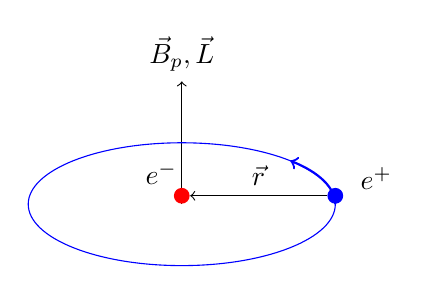
\begin{tikzpicture}[scale=1.3]
\draw[->](0,0) -- (0,1.2)node[above]{$\vec{B}_p,\vec{L}$};
\draw[blue] (0,0) ellipse (1.5 and .6);
\draw [->, thick,blue] (1.5,0) arc (0:45:1.5 and .6);
\node[fill=red,circle, minimum size=0.2cm,inner sep=0pt,above](em) at(0,0){};
\node at (-.2,.3){$e^-$};
\node[fill=blue,circle, minimum size=0.2cm,inner sep=0pt,above](pp) at(1.5,0){};
\node at (1.9,.25){$e^+$};
\draw[->] (pp) -- (em)node[above,midway]{$\vec{r}$};
\end{tikzpicture}
\end{marginfigure}
The hydrogen atom, from the electron's perspective, consists of a proton ``orbiting'' it. The ``orbiting'' proton generates a magnetic field which then interacts with the electron's spin. The potential energy of this {\em spin-orbit} interaction is
\beq
H_\rmt{so} = -\vec{\mu}_e\cdot\vec{B}_p.
\eeq
We model the magnetic field as the classical field generated by a moving charged particle $\vec{B}_p = \mu_0 I/(2r)$. The current is the electron charge divided by the classical orbital period $T_\rmt{orbit}$. However, the orbital period can be written in terms of of the angular momentum $L$ for a uniform circular motion model:
\beq
T_\rmt{orbit} = \frac{2\pi}{L}mr^2.
\eeq
So the magnetic field due to the classically orbiting proton is modeled as
\beq
\vec{B}_p = \frac{\mu_0 e \vec{L}}{4\pi m r^3} = \frac{e}{4\pi\epsilon_0 mc^2 r^3}\vec{L}.
\eeq\marginnote[-1cm]{We used $\epsilon_0\mu_0 = 1/c^2$ here.}%
We previously modeled the electron magnetic moment as being proportional to its spin, Eq.~(\ref{eq:dipolespin}):
\beq
\vec{\mu}_e = -\frac{e}{m}\vec{S}.
\eeq
We combine both of these to get the spin-orbit coupling energy perturbation operator
\beq
\hat{H}'_\rmt{so} = \left(\frac{e^2}{8\pi\epsilon_0} \right)\frac{1}{m^2c^2r^3} \hat{\vec{S}}\cdot\hat{\vec{L}}.
\eeq\marginnote[-1cm]{We are off by a factor of $1/2$ here - this factor is a correction due to the fact that the electron is not in an inertial reference frame. See AJP {\bf 57}, 171 (1989) for the details of this correction.}

Again we want to find the energy corrections due to this perturbation. We model this energy correction as a quantum operator and get the energy shift
\beq
E_\rmt{so} =\left(\frac{e^2}{8\pi\epsilon_0} \right)\frac{1}{m^2c^2} \bra{nlm_l}\frac{\hat{\vec{S}}\cdot{\hat{\vec{L}}}}{r^3}\ket{nlm_l}.
\label{eq:esofirst}
\eeq
The expectation value can be divided into two parts: the radial part and the spin-angular momentum part. We'll approach the spin-angular momentum part first.

\subsection{Combined Spin and Angular Momentum}
We previously introduced the idea of a combined spin-and-angular-momentum operator in Eq.~(\ref{eq:combinedangspin}),
\beq
\skew{4}\hat{\skew{4}\vec{\Ja}} = \hat{\vec{L}} + \hat{\vec{S}}.
\eeq
Squaring this, we get 
\beq
\Jh^2 = \hat{L}^2 + \hat{S}^2 + 2 \hat{\vec{S}}\cdot\hat{\vec{L}}
\eeq
which can be re-written to give us
\beq
\hat{\vec{S}}\cdot\hat{\vec{L}} = \frac{1}{2}\left(\Jh^2 - \hat{L}^2 - \hat{S}^2 \right).
\label{eq:sltoj}
\eeq
We now split up the energy eigenstate describing the electron into three parts: the radial piece, the orbital angular momentum piece, and the spin piece. This gives us:
\beq
\ket{\Psi_E} = \ket{\psi_r}\otimes\ket{lm_l}\otimes\ket{sm_s}.
\eeq
We know that
\bas
\bra{lm_l}\hat{L}^2\ket{lm_l} =& l(l+1)\hbar^2 \rmt{ and }\\
\bra{sm_s}\hat{S}^2\ket{sm_s} =& s(s+1)\hbar^2,
\eas
where $s=1/2$ for an electron. However, in order to determine the eigenvalues of the combined angular momentum operator, we need to change basis to the eigenstates of the $\Jh^2$ and $\Jh_z$ operators. This is done using the {\em Clebsch-Gordan coefficients}, best looked up in a table. The combined state is a sum of the separate eigenstates
\beq
\ket{jm_j} = \sum_{m_j = m_l + m_s}C_{m_lm_l;m_j}^{ls;j}\ket{lm_l}\otimes\ket{sm_s},
\label{eq:CGcoeff}
\eeq
where $j$ ranges from $\abs{l-s}$ to $(l+s)$ and $m_j$ ranges from $-j$ to $+j$ in integer steps. Once we've changed basis, then the eigenvalues are just
\beq
\bra{jm_j}\Jh^2\ket{jm_j} = j(j+1)\hbar^2.
\eeq%
\begin{example}
A hydrogen atom is the the quantum state $\ket{nlm_l} = \ket{31{-1}}$ with the electron in the $\ket{u}$ spin state. What is this state, written in the $\ket{jm_j}$ basis? What is the expectation value $\bra{31{-1}}\Jh^2\ket{31{-1}} $?

\model We model the hydrogen atom as a quantum system with the initial eigenstates from the Coulomb interaction model. We model the starting state as $l=1,m_l=-1,s=1/2,m_s=1/2$.

\vis With angular momentum of $l=1$ and $m_l=-1$, we could visualize the angular part of this wavefunction, though it doesn't really help us.

\sol We'll use the Clebsch-Gordan calculator online from  \href{http://www.wolframalpha.com/input/?i=Clebsch-Gordan+calculator}{Wolfram Alpha}. We have a range of $j_\rmt{max} = 3/2$ to $j_\rmt{min} = 1/2$. The possible states are thus
\beq
\ket{jm_j}=\begin{cases}j=3/2:&\ket{3/2,3/2}, \ket{3/2,1/2},\ket{3/2,-1/2},\ket{3/2,-3/2}\\
j=1/2:&\ket{1/2,1/2},\ket{1/2,-1/2}
\end{cases}
\eeq
Plugging in our inputs (where $j_1\rightarrow l$ and $j_2\rightarrow s$) we find only two non-zero entries in the $\ket{jm_j}$ basis:
\beq
\ket{1,{-1}}\otimes\ket{1/2,1/2} = \sqrt{\frac{1}{3}}\ket{3/2,-1/2} - \sqrt{\frac{2}{3}}\ket{1/2,-1/2}.
\eeq

The expectation value for $\Jh^2$ is thus
\bas
&\left(\sqrt{\frac{1}{3}}\bra{3/2,-1/2} - \sqrt{\frac{2}{3}}\bra{1/2,-1/2}\right)\Jh^2\left(\sqrt{\frac{1}{3}}\ket{3/2,-1/2} - \sqrt{\frac{2}{3}}\ket{1/2,-1/2}\right)\\
&=\frac{1}{3}\left[\frac{3}{2}\left(\frac{3}{2} + 1 \right)\right]\hbar^2 + \frac{2}{3}\left[\frac{1}{2}\left(\frac{1}{2} + 1 \right)\right]\hbar^2=\frac{7}{4}\hbar^2.
\eas

\assess This has the correct units. And it is in the right range, since the expectation value for $\hat{L}^2$ is $2\hbar^2$ and the $z$-component of the angular momentum is anti-parallel to the electron spin.

\end{example}

Once we write the state in the $\ket{jm_j}$ basis, we can evaluate the angular piece of the energy shift, Eq.~(\ref{eq:esofirst}). We get
\beq
\left(\bra{lm_l}\otimes\bra{sm_s}\right)\hat{\vec{S}}\cdot{\hat{\vec{L}}}\left(\ket{lm_l}\otimes\ket{sm_s}\right) = \frac{\hbar^2}{2}\left[j(j+1) -l(l+1) - s(s+1)\right]
\label{eq:lmlsexpec}
\eeq
where we used Eq.~(\ref{eq:sltoj}) to re-write the dot product. 
\subsection{Radial Component Shift}
We next deal with the radial piece. We need to know the expectation value for $1/r^3$. Because we know the expectation value for $1/r^2$, Eq.~(\ref{eq:oneoverrsq}), we can use another trick to relate that to the expectation value for $1/r^3$.
\begin{exercise}
Another useful relationship, known as {\em Kramers' relation} lets us relate the expectation values for the powers of $r$. The relationship is, for power $k$ and eigenfunction $\psi_{nlm_l}$
\beq
\frac{k+1}{n^2}\avg{\hat{R}^k} - (2k+1)a_0\avg{\hat{R}^{k-1}} + \frac{k}{4}\left[(2l+1)^2-k^2\right]a_0^2\avg{\hat{R}^{k-2}}=0.
\eeq
Show that, given the expectation value for $1/r^2$, the expectation value for $1/r^3$ is
\beq
\avg{\frac{1}{\hat{R}^3}} = \frac{1}{l(l+1/2)(l+1)n^3a_0^3}.
\label{eq:oneoverrcube}
\eeq

\end{exercise}

With the expectation values from Eq.~(\ref{eq:oneoverrcube}) and from Eq.~(\ref{eq:lmlsexpec}), we find that the energy shift for the spin-orbit coupling is\arnote{Fill in the missing steps to get the constants all straightened out.}%
\bas
E_\rmt{so} =&\left(\frac{e^2}{8\pi\epsilon_0} \right)\frac{1}{m^2c^2} \frac{(\hbar^2/2)\left[j(j+1) - l(l+1) - s(s+1)\right]}{l(l+1/2)(l+1)n^3a_0^3} \\
=& \frac{E_n^2}{mc^2} \frac{n\left[j(j+1) - l(l+1) - s(s+1)\right]}{l(l+1/2)(l+1)}\label{eq:esofinal}
\eas
This is on the same order of magnitude as the relativistic correction from Eq.~(\ref{eq:erelfinal}). We combine the two corrections (and noting that $s=1/2$) to give a total fine-structure correction of
\beq
E_\rmt{fs} = \frac{E_n^2}{2mc^2}\left(3-\frac{4n}{j+1/2}\right).
\eeq
\begin{exercise}
Repeat your calculations for the energy shifts in the Balmer series from Exercise \ref{ex:balermred}, this time including the total fine structure shift, not just the relativistic shift. How much different are they? Modern laser spectroscopy has a resolution of around $0.1$~Hz. Can we distinguish between these two models? 
\end{exercise}



%---------------------------------------
\chapter{Zeeman Effect and Hyperfine Splitting}
\begin{marginfigure}
\centering
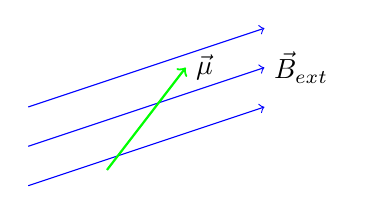
\begin{tikzpicture}[scale=1]
\draw[->,blue] (0,0) -- (3,1);
\draw[->,blue] (0,0.5) -- (3,1.5) node[right,black]{$\vec{B}_\rmt{ext}$};
\draw[->,blue] (0,1) -- (3,2);
\draw[->,green,thick] (1,0.2) -- (2,1.5) node[right,black]{$\vec{\mu}$};

\end{tikzpicture}
\end{marginfigure}
We now model what happens when we apply an external magnetic field to a hydrogen atom. The atom has a magnetic dipole moment that is modeled with two components: the orbital angular momentum and the spin dipole moments, $\vec{\mu}=\vec{\mu}_l + \vec{\mu}_s$. The potential energy of the magnetic dipole in an external magnetic field is $U = -\vec{\mu}\cdot\vec{B}_\rmt{ext}$. We model this energy as a perturbation to the Coulomb interaction energy eigenvalues and eigenstates,
\beq
H'_\rmt{Z} = -\left(\vec{\mu}_l + \vec{\mu}_s\right)\cdot\vec{B}_\rmt{ext}
\eeq
where we write the magnetic dipole moments as
\beq
\vec{\mu}_l = -\frac{e}{2m}\vec{L} \rmt{ and } \vec{\mu}_s = g\left(\frac{-e}{2m}\right)\vec{S} = -\frac{e}{m}\vec{S}
\eeq
with Land\'{e} $g$-factor set to $2$ for the electron. So the Hamiltonian perturbation is
\beq
\hat{H}'_\rmt{Z} = \frac{e}{2m}\left(\hat{\vec{L}} + 2\hat{\vec{S}}\right)\cdot\vec{B}_\rmt{ext}.
\label{eq:zeemanpert}
\eeq
As we saw in Section \ref{sec:socoupling}, there is an internal magnetic field that interacts with the electron. Depending on the strength of the external magnetic field, we need to model the perturbation as affecting the $\ket{lm_l}$ states (for $\vec{B}_\rmt{ext} \gg \vec{B}_\rmt{int}$) or as a perturbation of the $\ket{jm_j}$ states for $\vec{B}_\rmt{ext} \ll \vec{B}_\rmt{int}$. We will treat these two cases separately.\marginnote{There is another model that smoothly joins these two limits, but we will not be discussing that here.}

\section{Strong-Field Zeeman Splitting}

We first treat the case where the external magnetic field is large: $\vec{B}_\rmt{ext} \gg \vec{B}_\rmt{int}$. In this model, we will treat the fine structure splitting as a perturbation of the eigenstates of the magnetic field interaction. So the first perturbation we treat from the Coulomb interaction eigenstates is Eq.~(\ref{eq:zeemanpert}). We will orient our model so that the magnetic field points along the $z$-direction: $\vec{B}_\rmt{ext} = B_\rmt{ext}\hat{z}$. The interaction operator is then
\beq
\hat{H}'_\rmt{Z} = \frac{e B_\rmt{ext}}{2m}\left(\hat{L}_z + 2\hat{S}_z\right).
\eeq
The energy shift due to this perturbation is just
\beq
E_\rmt{Z} = \frac{e B_\rmt{ext}}{2m}\left(m_l + 2m_s\right).
\eeq
This shift breaks the energy degeneracy of the $m_l$ and $m_s$ states and is linear in the external magnetic field strength. At this point we return to the fine structure model and add in those perturbations if we want a more accurate model. However, depending on the size of the external magnetic field, we may not need to add those models to get good agreement with experiment.

\begin{exercise}
What are the energies of the eight $n=2$ hydrogen states under the strong-field Zeeman splitting. Ignoring the fine-structure, how many distinct levels are there and what are their degeneracies?

\end{exercise}

\section{Weak-Field Zeeman Splitting}

We next treat the case where the external magnetic field is small compared to the internal magnetic field: $\vec{B}_\rmt{ext} \ll \vec{B}_\rmt{int}$. As we saw in Section \ref{sec:socoupling}, the eigenstates we should use are the $\ket{jm_j}$ states. So the first step is to use re-write any state in terms of its $j$ and $m_j$ components using the Clebsch-Gordan coefficients, Eq.~(\ref{eq:CGcoeff}). In this basis, the energy shift due to the perturbation Hamiltonian, Eq.~(\ref{eq:zeemanpert}) is
\beq
E_\rmt{Z} = \bra{njm_j}\hat{H}'_\rmt{Z}\ket{njm_j} = \frac{e}{2m}\vec{B}_\rmt{ext}\cdot\avg{\hat{\vec{L}} + 2\hat{\vec{S}}} = \frac{e}{2m}\vec{B}_\rmt{ext}\cdot\avg{\skew{4}\hat{\skew{4}\vec{\Ja}}+ \hat{\vec{S}}}
\eeq
where we used the definition of the combined orbital and spin angular momentum from Eq.~(\ref{eq:combinedangspin}). We find the average value for the spin operator by modeling the total angular momentum $\Jv$ as constant where the orbital angular momentum and the spin angular momentum precess rapidly around it.%
\begin{marginfigure}
\centering
\begin{tikzpicture}[scale=1.3]
\begin{scope}[shift={(1.1,1.65)}]
\draw[rotate=-30] (0,0) ellipse (1.2 and .3);
\end{scope}
\node[fill=magenta,circle, minimum size=0.1cm,inner sep=0pt,above](em2) at (1.1,1.65){};
\begin{scope}[shift={(-.2,.2)}]
\draw[->,magenta,thick](1.1,1.65) -- (2,3) node[midway,left,black]{$\vec{S}\cdot\Jv$};
\end{scope}
\node[fill=blue,circle, minimum size=0.2cm,inner sep=0pt,above](em1) at(0,0){};
\draw[->,blue,thick](em1) -- (2,3) node[near start,left,black]{$\Jv$};
\node[fill=red,circle, minimum size=0.2cm,inner sep=0pt,above](A) at (2.2,.9){};
\draw[->,red,thick](em) -- (A)node[midway,below,black]{$\vec{L}$};
\draw[->,green,thick] (A) --(2,3) node[midway,right,black]{$\vec{S}$};

\end{tikzpicture}
\end{marginfigure}%
The projection of $\vec{S}$ onto $\Jv$ is 
\beq
\vec{S}_\rmt{avg} = \frac{\vec{S}\cdot\Jv}{\Ja^2}\Jv
\eeq
so the average value of the vector sum becomes
\beq
\avg{\skew{4}\hat{\skew{4}\vec{\Ja}}+ \hat{\vec{S}}} = \avg{\left(1 + \frac{\vec{S}\cdot\Jv}{\Ja^2}\right) \skew{4}\hat{\Jv}}.
\eeq
Furthermore, because $\hat{L}^2 = \Ja^2 + \hat{S}^2 - 2\hat{\vec{S}}\cdot\skew{4}\hat{\Jv} $, the average of the dot product is 
\beq
\avg{\hat{\vec{S}}\cdot\skew{4}\hat{\Jv}} = \frac{\hbar^2}{2}\left[j(j+1) + s(s+1) - l(l+1)\right].
\eeq\arnote[-1cm]{I skipped a couple of steps here. Fill them in.}
Putting these together we get the weak-field Zeeman shift for a magnetic field oriented along the $z$-direction of 
\bas
E_\rmt{Z} = & \frac{e}{2m}\left[1+ \frac{j(j+1) - l(l+1) + s(s+1)}{2j(j+1)} \right]B_\rmt{ext}\avg{\Jh_z}\\
=& \frac{e\hbar}{2m}g B_\rmt{ext}m_j,
\label{eq:weakfieldzeeman}
\eas
where the term in the square brackets is known as the Land\'{e} $g$-factor. 

\begin{example}
What is the energy splitting for the ground state of hydrogen due to the weak-field Zeeman effect?

\model We'll model the external magnetic field as much smaller than the internal field and use the energy shift we found in Eq.~(\ref{eq:weakfieldzeeman}).

\vis We assume the magnetic field is aligned along the $z$-direction.

\sol The ground state is modeled as $\ket{nlm_l} = \ket{100}$ so $l=0$ and the electron could be in either spin state: $s=1/2$, $m_s = \pm 1/2$. So the combined state gives us $j=1/2$ and $m_j = \pm 1/2$. That means the Land\'{e} $g$-factor is 
\beq
g=\left[1+ \frac{j(j+1) - l(l+1) + s(s+1)}{2j(j+1)} \right] = 1 + \frac{3/4 - 0 + 3/4}{2\cdot 3/4} = 2.
\eeq
So the energy shift is
\beq
E_\rmt{Z} = \pm\frac{e\hbar}{2m}B_\rmt{ext}.
\eeq

\assess The energy shift scale is known as the {\em Bohr magneton}
\beq
\mu_B \equiv \frac{e\hbar}{2m} = 5.788\times 10^{-5} \;\rmt{ eV/T}.
\eeq
So the scale of the shift is small for a magnetic field of a few tens of mT. The Land\'{e} $g$-factor is $2$ which is what we've seen previously for an electron. 

\end{example}

\begin{exercise}
What are the energies of the eight $n=2$ hydrogen states under the weak-field Zeeman splitting. Ignoring the fine-structure, how many distinct levels are there and what are their degeneracies? Plot each state with its appropriate slope as a function of $\mu_B B_\rmt{ext}$

\end{exercise}

\section{Hyerfine Splitting}

We treat one more perturbation model for the hydrogen atom. We model the spin $\vec{I}$ of the nucleus (in this case a single proton) as a magnetic dipole moment where
\beq
\vec{\mu}_N = \frac{g_p e}{2m_p}\vec{I} \rmt{ where } g_p = 5.59.
\eeq
We are specifically interested in the case where the electron wavefunction overlaps the nucleus --- where $r=0$. Those states, from Figure \ref{fig:rplots3}, all  have angular momentum quantum numbers $l=0$. We therefore model the nucleus as a uniformly magnetized sphere and look at the magnetic field inside the sphere in order to find the magnetic field as $r\rightarrow 0$.

\begin{marginfigure}
\centering
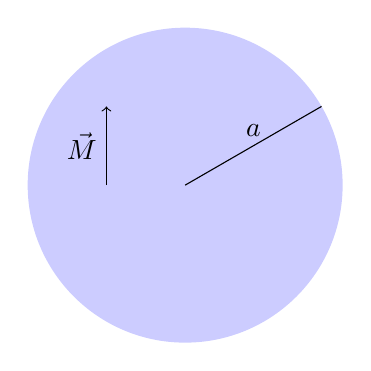
\begin{tikzpicture}
\fill[fill=blue!20] (0,0) circle (2);
\draw (0,0)--(30:2) node[midway,above]{$a$};
\draw[->](-1,0) -- (-1,1)node[midway,left]{$\vec{M}$};
\end{tikzpicture}
\end{marginfigure}

The magnetic dipole for a sphere of uniform magnetization $\vec{M}$ is
\beq
\vec{\mu} = \frac{4}{3}\pi a^3\vec{M}.
\eeq
The constant magnetic field inside a uniformly magnetized sphere is 
\beq
\vec{B}_\rmt{inside}(\vec{r}) = \frac{\mu_0}{2\pi}\frac{\vec{\mu}}{a^3},
\eeq
so the total magnetic field inside the sphere is
\beq
\vec{B}_N = \int \vec{B}_\rmt{inside}dV = \frac{\mu_0}{2\pi} \frac{\vec{\mu}}{a^3} \left(\frac{4}{3}\pi a^3 \right) = \frac{2}{3}\mu_0 \vec{\mu}_N.
\eeq
So we now model the interaction Hamiltonian for the $l=0$ states at $r=0$ as the interaction between the electron's dipole moment and the magnetic field due to the nuclear spin where $U = -\vec{\mu}\cdot\vec{B}$. The interaction Hamiltonian is therefore\arnote{I've skipped steps - put them all together in your notes. I've left the spin dipoles in terms of the Land\'{e} $g$-factors.}
\beq
\hat{H}'_\rmt{hf} = \frac{2}{3}\frac{g_e e}{2 m_e}\frac{\mu_0 g_p e}{2m_p}\left(\hat{\vec{S}}\cdot\hat{\vec{I}}\right).
\eeq
We now use the same technique as in Section \ref{sec:socoupling} for the spin-orbit coupling model. We write the total spin (electron plus nucleus) as $\vec{F} = \vec{S} + \vec{I}$, from Eq.~(\ref{eq:nucleartotalspin}), so that $\vec{S}\cdot\vec{I} = (F^2 - S^2 - I^2)/2$. In this case, the interaction Hamiltonian is \arnote{Fill in these skipped steps, too.}
\beq
\hat{H}'_\rmt{hf} =\frac{1}{12} \frac{\mu_0 g_e g_p e^2}{m_p m_e}\left(\hat{F}^2 - \hat{S}^2 - \hat{I}^2\right).
\eeq
Therefore, the energy shift due to this interaction, known as the {\em hyperfine splitting} is 
\beq
E_\rmt{hf} = \frac{1}{12} \frac{\mu_0 g_e g_p e^2}{m_p m_e}\bra{\psi_{n00}(\vec{r}=0)}\left(\hat{F}^2 - \hat{S}^2 - \hat{I}^2\right)\ket{\psi_{n00}(\vec{r}=0)}
\eeq
for states $\ket{\psi_{nlm_l}}$ where $l=0$ and $m_l=0$.
\begin{example}
What is the hyperfine splitting for the $\ket{nlm_l} = \ket{100}$ states of the hydrogen atom?

\model We'll use the Coulomb interaction model as the base states for this calculation. We'll model the hyperfine splitting as a small perturbation of the base energy.

\vis There are two sets of possibilities when we combine spin states: the electron and nuclear spins could be aligned or anti-aligned. If the spins are aligned, we have a spin triplet where the total spin is $f=1$ and $m_f = -1,0,1$. If the spins are anti-aligned we have the singlet state $f=0$ and $m_f=0$. 

\sol So we have two cases to treat: the $f=1$ and $f=0$ cases. In either case, the total electron and nuclear spins are unchanged and 
\beq
\avg{\hat{S}^2} = \frac{3}{4}\hbar^2 \rmt{ and } \avg{\hat{I}^2} = \frac{3}{4}\hbar^2.
\eeq
If $f=1$ then $\avg{\hat{F}^2} = 2\hbar^2$. If $f=0$ then $\avg{\hat{F}^2}=0$. So the energies of our two states are
\beq
E_\rmt{hf} = \frac{1}{12} \frac{\mu_0 g_e g_p e^2}{m_p m_e} \abs{\psi_{100}(\vec{r}=0)}^2\left[\underbrace{\left(\begin{aligned}2&\\0&\end{aligned}\right)}_{\rmt{for } f=1,0} -\frac{3}{4} - \frac{3}{4} \right]\hbar^2.
\eeq
The quantity in the square brackets is either $-3/2$ or $+1/2$. We also calculate the magnitude of the wavefunction, evaluated at $\vec{r}=0$ using the radial wavefunction from Table \ref{table:rwave} and the angular wavefunction from Table \ref{table:sphar}. This gives us $\abs{\psi_{100}(\vec{r}=0)}^2 = 1/(\pi a_0^3)$. So the energy difference between these two states is\arnote{More skipped steps to fill in!}
\beq
\Delta E_\rmt{hf} = \frac{2 g_p g_e \hbar^4}{3 m_p m_e^2 c^2a_0^4}.
\eeq

\assess If a transition happens between these hyperfine energies, then there will be emitted ElMaWs with that energy. That corresponds to a frequency ($\nu =\Delta E/h$) of $1420$~MHz, a commonly measured frequency in astrophysics.

\end{example}

\begin{exercise}
What is the hyperfine splitting (in terms of the frequency of the emitted ElMaW) for muonic hydrogen in which a muon -- same charge and $g$-factor as the electron but 207 times the mass -- substitutes for an electron in an atom?
\end{exercise}

\begin{exercise}
Calculate the hyperfine splitting for $j=1/2$ fine structure states for the $n=2$ hydrogen states.  Model them as perturbations of the fine-structure states shown in Fig. \ref{fig:hhyperfine}. Report the splitting in terms of the ground state hyperfine splitting energy.
\begin{figure}
\begin{tikzpicture}
\draw (0,0) -- (2,0)node[above,near start, align=right]{$n=1,l=0$};
\draw (3,0) -- (5,0)node[above,near start]{$j=1/2$};
\draw (6,.4) -- (8,.4)node[above,near start]{$f=1$};
\draw (6,-.4) -- (8,-.4)node[above,near start]{$f=0$};

\draw (0,3) -- (2,3)node[above,near start, align=left]{$n=2,l=0$};
\draw (3,4.0)-- (5,4.0)node[above,near start]{$j=3/2$};
\draw (3,2.4)-- (5,2.4)node[above,near start]{$j=1/2$};
\draw (6,4.3) -- (8,4.3)node[above,near start]{$f=2$};
\draw (6,3.7) -- (8,3.7)node[above,near start]{$f=1$};
\draw (6,2.7) -- (8,2.7)node[above,near start]{$f=1$};
\draw (6,2.1) -- (8,2.1)node[above,near start]{$f=0$};
\node[align=left] at (4,5){Fine Structure};
\node[align=left] at (7,5){Hyperfine Structure};
\caption[][3cm]{Hyperfine structure for hydrogen.}
\label{fig:hhyperfine}
\end{tikzpicture}
\end{figure}
\end{exercise}


%---------------------------------------
\chapter{Atomic transitions}

We now model transitions between energy eigenstates of the hydrogen atom. The first element of our model will be a small external magnetic field oriented along the $z$-direction. This breaks the degeneracy of the $m_l$ states and provides an relative axis for our incoming ElMaW polarization. We send in an ElMaW with an arbitrary polarization of the wave oriented in the $\vec{r}$ direction. We need to calculate the matrix elements given by the dipole transition model Eq.~(\ref{eq:hjkdipole}) from Section \ref{sec:dipoletrans}
\beq
H'_{jk} = \bra{\psi_j}\hat{H}'\ket{\psi_k} = e\bra{\psi_j}\hat{\vec{R}}\ket{\psi_k}\left(-E_0\cos\omega t\right)
\eeq
in order to determine which transitions will happen and their oscillator strengths. We model the eigenstates using the Coulomb interaction model from Section \ref{sec:hydrogenstates}. The states in the position basis are represented by the wavefunctions Eq.~(\ref{eq:totalwavefunction})
\beq
\Psi_{nlm_l}(r,\theta,\phi) = R_{nl}(r)\Ylm(\theta,\phi)
\eeq
where
\beq
R_{nl}(r) = \sqrt{\left(\frac{2}{n a_0}\right)^3\frac{(n-l-1)!}{2n\left[(n+l)!\right]^3}}\E{-\frac{r}{na_0}}\left(\frac{2r}{na_0}\right)^l L_{n-l-1}^{2l+1}\left(\frac{2r}{na_0}\right)
\eeq\marginnote[-1cm]{Some \CAS do not calculate the Laguerre polynomials with the same normalization as we need. You may need to multiply this by a factor of $(n+l)!$ to get the normalization correct. Always double-check this!}
and
\beq
\Ylm(\theta,\phi)=\sqrt{\frac{(2l+1)(l-m_l)!}{4\pi(l+m_l)!}} P_l^{m_l}(\cos\theta) \E{\I m_l\phi}.
\eeq
Because we are working in spherical coordinates, the our model of the dipole operator $\hat{\vec{R}}$ needs to be written in spherical coordinates. We make this conversion to the operator in the position basis as
\beq
\hat{\vec{R}} \rightarrow \begin{cases}
x =& r \sin\theta\cos\phi\\
y =& r \sin\theta\sin\phi\\
z =& r \cos\theta
\end{cases}
\eeq
\begin{marginfigure}
\centering
\begin{tikzpicture}[scale=1.3]
\draw[->](0,0,0) -- (2,0,0)node[right]{$y$};
\draw[->](0,0,0) -- (0,2,0)node[right]{$z$};
\draw[->](0,0,0) -- (0,0,2)node[right]{$x$};
\draw[->,thick](0,0,0) -- (1.5,1,0.8)node[above,midway]{$r$};
\draw[dashed] (0,0,0) -- (1.5,0,.8);
\begin{scope}[rotate around={30:(0,0)}]
    \draw (0:0.5) arc (0:62:0.5)node[midway,above]{$\theta$};
\end{scope}
\begin{scope}[canvas is xz plane at y=0, rotate around={90:(0,0)}]
    \draw (0:0.5) arc (0:-62:0.5)node[midway,below]{$\phi$};
\end{scope}
\draw[dashed] (1.5,1,0.8) -- (1.5,0,.8);
\draw[dashed] (0,0,.8) -- (1.5,0,.8);
\draw[dashed] (1.5,0,0) -- (1.5,0,.8);
\end{tikzpicture}
\end{marginfigure}%
The matrix elements which determine the transitions and oscillator strengths between the two different states $\ket{\Psi_{nlm_l}}$ and $\ket{\Psi_{n'l'm'_l}}$ are, in the position basis,
\begin{multline}
\bra{\Psi_{nlm_l}}\hat{H}'\ket{\Psi_{n'l'm'_l}} =\\ \int\displaylimits_0^\infty r^2 dr\int\displaylimits_0^\pi \sin\theta d\theta \int\displaylimits_0^{2\pi}d\phi\;\Psi^*_{nlm_l}(r,\theta,\phi) \;\vec{r}\; \Psi^{}_{n'l'm'_l}(r,\theta,\phi).
\label{eq:matrixintegral2}
\end{multline}
We will directly calculate some of these later, but we can use a few tricks to narrow down all the possible transitions, simplifying the work we do later.

\section{$m_l$ Selection Rules}
We need to orient the incoming ElMaW that is driving the dipole transitions before we can use our tricks. We will start by orienting the external magnetic field along the $z$-axis and then orient the ElMaW polarization so that it also points along the $z$-axis.
\begin{marginfigure}
\centering
\begin{tikzpicture}[scale=3]
\draw[->](0,0,0) -- (.6,0,0)node[right]{$z$};
\draw[->](0,0,0) -- (0,.5,0)node[right]{$x$};
\draw[->](0,0,0) -- (0,0,2)node[right]{$y$};
\draw[->,thick,red](-0.5,0,0) -- (.5,0,0)node[above,black]{$\vec{B}_\rmt{ext}$};
\begin{scope}[canvas is xz plane at y=0,shift={(0,0,0)}]
\draw[blue,->,decorate, decoration={snake,amplitude=10,segment length=20, post length=.04cm}](0,2)--(0,.2) node[midway, above,shift=({-.5,0}),black]{$\vec{E}$};
\draw[<->,thick,blue](-.2,.6)--(.2,.6);
\end{scope}
\end{tikzpicture}
\end{marginfigure}%
For this model, the relevant matrix element is then
\beq
\bra{\Psi_{nlm_l}}\hat{Z}\ket{\Psi_{n'l'm'_l}}.
\eeq
The trick we will use is that the commutation relationship between $\com{\hat{L}_z,\hat{Z}}=0$. 

\begin{exercise}
Using the operator algebra from Eqs.~(\ref{XP commute}) and (\ref{eq:ldefinition}) to show that
\beq
\begin{aligned}
\com{\hat{L}_x,\hat{X}} =& 0 & \com{\hat{L}_y,\hat{X}} =& -\I\hbar \hat{Z} & \com{\hat{L}_z,\hat{X}} =& \I\hbar \hat{Y}\\
\com{\hat{L}_x,\hat{Y}} =&\I\hbar \hat{Z}  & \com{\hat{L}_y,\hat{Y}} =& 0 & \com{\hat{L}_z,\hat{Y}} =& -\I\hbar \hat{X}\\
\com{\hat{L}_x,\hat{Z}} =& -\I\hbar\hat{Y} & \com{\hat{L}_y,\hat{Z}} =& \I\hbar \hat{X} & \com{\hat{L}_z,\hat{Z}} =& 0
\end{aligned}
\label{eq:lzcomwithxyz}
\eeq \marginnote[-3cm]{Note that when the commutators are in the cyclic permutation $xyz$, $yzx$, or $zxy$, the result is positive and when you switch any two indices of these, you get a negative result. This can be written neatly using the Levi-Civita symbol $\varepsilon_{ijk}$: $\com{\hat{L}_i,\hat{X}_j}= \I\hbar\hat{X}_k\varepsilon_{ijk}$.}
\end{exercise}
What we now look at is the matrix element
\bas
0=&\bra{\Psi_{nlm_l}}\com{\hat{L}_z,\hat{Z}}\ket{\Psi_{n'l'm'_l}}\\
&=\hbar\left(m_l - m'_l\right)\bra{\Psi_{nlm_l}}\hat{Z}\ket{\Psi_{n'l'm'_l}}
\eas\arnote[-1.5cm]{Fill in the missing steps using the eigenvalue equation for $\hat{L}_z$ and the fact that it is a Hermitian operator.}%
So either the matrix element is zero or $m_l = m'_l$ for this transition. This type of transition is known as a {\em $\pi$-transition} where $\Delta m_l = m_l - m'_l = 0$. Furthermore, this same procedure applies if we add in the fine structure or the hyperfine structure models --- the selection rule for a $\pi$-transition is $\Delta m_j = 0$ or $\Delta m_f = 0$ for those models.

Instead of orienting the ElMaW polarization along the magnetic field and the wave perpendicular to the magnetic field, we can also orient the wave propagation along the magnetic field and give the ElMaW circular polarization as we did in Section \ref{sec:ybasis}. 
\begin{marginfigure}
\centering
\begin{tikzpicture}[scale=3]
\draw[->](0,0,0) -- (.6,0,0)node[right]{$z$};
\draw[->](0,0,0) -- (0,.5,0)node[right]{$x$};
\draw[->](0,0,0) -- (0,0,1)node[right]{$y$};
\draw[->,thick,red](-0.1,0,0) -- (.5,0,0)node[above,black]{$\vec{B}_\rmt{ext}$};
\begin{scope}[canvas is yz plane at x=-.5,shift={(0,0,0)}]
\draw[<-,thick,blue] (10:.2) arc (10:360:.2)node[midway,black,below]{$\vec{E}$};
\end{scope}
\draw[->,thick,blue](-.5,0,0)--(-.1,0,0);
\end{tikzpicture}
\end{marginfigure}%
The electric field polarization for right- and left-handed circular polarization is (in terms of the 3-vector unit vectors)
\bas
\rmt{right-handed: }& \hat{x} + \I \hat{y}\\
\rmt{left-handed: }&\hat{x} - \I \hat{y}.
\eas
Modeling the interaction as we did before, we now want the matrix elements
\beq
\bra{\Psi_{nlm_l}}\hat{X} \pm \I \hat{Y}\ket{\Psi_{n'l'm'_l}}.
\eeq
We use the same trick as before, looking at the commutator between $\hat{L}_z$ and $\hat{X} \pm \I \hat{Y}$:
\beq
\bra{\Psi_{nlm_l}}\com{\hat{L}_z,\hat{X} \pm \I \hat{Y}}\ket{\Psi_{n'l'm'_l}}=\hbar\left(m_l - m'_l\right)\bra{\Psi_{nlm_l}}\hat{X} \pm \I \hat{Y}\ket{\Psi_{n'l'm'_l}}.
\eeq\arnote[-1cm]{Fill in the missing steps.}
However, we also can expand the commutator, using the relationships from Eq.~(\ref{eq:lzcomwithxyz}). This gives us
\beq
\com{\hat{L}_z,\hat{X} \pm \I \hat{Y}} = \pm\hbar\left(\hat{X} \pm \I \hat{Y}\right).
\eeq\arnote[-1cm]{more missing steps.}
So, inserting this into the matrix element, we get
\beq
\bra{\Psi_{nlm_l}}\com{\hat{L}_z,\hat{X} \pm \I \hat{Y}}\ket{\Psi_{n'l'm'_l}}=\pm\hbar\bra{\Psi_{nlm_l}}\hat{X} \pm \I \hat{Y}\ket{\Psi_{n'l'm'_l}}
\eeq
or, in other words, $\Delta m_l = \pm 1$ for right- and left-handed circular polarization. These transitions are known as {\em $\sigma_\pm$}-transitions. These also represent a conservation of angular momentum. The incoming ElMaW with circular polarization has angular momentum of $\hbar$ and it transfers that angular momentum to the hydrogen atom through the interaction.

\section{$l$ Selection Rules}

We are going to use a similar set of tricks to determine the selection rules for $\Delta l = l - l'$. We first need a couple of commutation relationships.

\begin{exercise}
Show that
\bas
\com{\hat{L}^2,\hat{X}} = &2\I\hbar\left(\hat{Y}\hat{L}_z - \hat{Z}\hat{L}_y - \I\hbar \hat{X}\right)\\
\com{\hat{L}^2,\hat{Y}} = &2\I\hbar\left(\hat{Z}\hat{L}_x - \hat{X}\hat{L}_z - \I\hbar \hat{Y}\right)\\
\com{\hat{L}^2,\hat{Z}} = &2\I\hbar\left(\hat{X}\hat{L}_y - \hat{Y}\hat{L}_x - \I\hbar \hat{Z}\right).
\eas

\end{exercise}

And one more set of relationships:
\begin{exercise}
Show that
\beq
\com{\hat{L}^2,\com{\hat{L}^2,\hat{Z}}} = 2\hbar^2\left(\hat{L}^2\hat{Z} + \hat{Z}\hat{L}^2\right).
\label{eq:lsquaredsquared}
\eeq\marginnote[-2cm]{You also need the fact that $\vec{r}\cdot\vec{L} = 0$ since the angular momentum is always perpendicular to the position and momentum.}
\end{exercise}

We finally extend Eq.~(\ref{eq:lsquaredsquared}) to all three directions, giving us
\beq
\com{\hat{L}^2,\com{\hat{L}^2,\hat{\vec{R}}}} = 2\hbar^2\left(\hat{L}^2\hat{\vec{R}} + \hat{\vec{R}}\hat{L}^2\right).
\label{eq:lsquaredexpanded}
\eeq\arnote[-1cm]{Write this out and make sure you know how to extend this.}

We now use the same trick as last time, looking at the matrix elements around this commutator.
\beq
\bra{\Psi_{nlm_l}}\com{\hat{L}^2,\com{\hat{L}^2,\hat{\vec{R}}}} \ket{\Psi_{n'l'm'_l}}.
\eeq
One the one hand, we evaluate this using the eigenvalues of $\hat{L}^2$ and get
\beq
\hbar^4\left[l(l+1) - l'(l'+1)\right]^2\bra{\Psi_{nlm_l}}\hat{\vec{R}} \ket{\Psi_{n'l'm'_l}}.
\eeq\arnote[-1cm]{More to work out!}
On the other hand, we expand the commutator using Eq.~(\ref{eq:lsquaredexpanded}) and get
\beq
2\hbar^4\left[l(l+1) + l'(l'+1)\right]\bra{\Psi_{nlm_l}}\hat{\vec{R}} \ket{\Psi_{n'l'm'_l}}.
\eeq\arnote[-1cm]{You need to do this one, too.}
Comparing these two, we find that either the matrix element is zero or
\beq
\left[l(l+1) - l'(l'+1)\right]^2 = 2\left[l(l+1) + l'(l'+1)\right].
\eeq
There are four possible solutions to this:
\bas
l =& -2-l' \rightarrow \rmt{ no good since }l,l'>0\\
l=& l' -1 \rightarrow \rmt{ or } \Delta l = +1\\
l=& l' +1 \rightarrow \rmt{ or } \Delta l = -1\\
l=&-l' \rightarrow \rmt{ also no good}.
\eas
This selection rule then means that $\Delta l = \pm1$. This selection rule also reflects the conservation of angular momentum as momentum is transferred from the ElMaW to the atom.

If we include the fine structure or hyperfine structure in our model, the selection rule changes a bit. For those two models, there are three allowable transitions: $\Delta j = 0,\pm 1$ and $\Delta f = 0, \pm 1$. This is because we have to include the spin and that additional degree of freedom expands the possibility. Only for $j=j'=0$ is the transition not going to happen (since this case has zero net spin). The same applies for transitions in the hypefine structure model: the $f = 0 \rightarrow f'=0$ transitions do not happen.

\section{Brute-force calculations}

These tricks have helped us narrow down the number of possible transitions. However, to actually calculate the transition probabilities, we need to do the integral in Eq.~(\ref{eq:matrixintegral2}). This is straight-forward using a \CAS and is left for an exercise.

\begin{exercise}
Calculate the first 10 allowable transition matrix elements for the Coulomb interaction hydrogen model for $\pi$ and $\sigma_\pm$ transitions.
\end{exercise}


%---------------------------------------
\chapter{Modeling Bound States Numerically}

We have looked at a number of models where the TISWEs have analytic solutions. We now want to look at techniques for modeling systems that do not fit into this same neat package. We will use the same general Technique \ref{tactis:TISWEBC}, adapted to using numerical techniques.

\section{Scaling the TISWE to dimensionless parameters}

As before, we will model our system as a time-independent Hamiltonian using the potential model of interest. The next step is to determine the TISWE for the coordinates of the system. At this point we previously looked up the solution to the second-order differential equation. However, in order to find a numerical solution, it makes sense to re-write the TISWE using dimensionless parameters. That makes the numerical calculations easier--- we will typically be dealing with counting numbers and other ``nice'' values instead of large or small decimal numbers. We'll practice turning a TISWE into dimensionless parameters as an example.

\begin{example}
What is the TISWE for the infinite potential well model in dimensionless parameters?

\model We'll model our system as a matter wave in an infinite box of length $L$ centered on $x=0$. As before, the potential will be zero in the box and infinite outside the box.

\vis Our potential well looks the same as it did before, Figure \ref{fig:infwell2}.
\begin{figure}
\centering
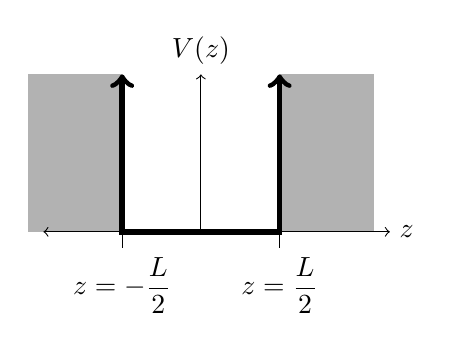
\begin{tikzpicture}
\fill[black!30] (-2.2,0) rectangle +(1.2,2);
\fill[black!30] (1,0) rectangle +(1.2,2);
\draw[<->](-2,0) -- (2.4,0)node[right]{$z$};
\draw[->](0,0) -- (0,2)node[above]{$V(z)$};

\draw[line width=2pt,<->](-1,2) -- (-1,0) -- (1,0) -- (1,2);

\draw (-1,0) -- (-1,-.2) node[below,align=center] {$\displaystyle z=-\frac{L}{2}$};
\draw (1,0) -- (1,-.2) node[below,align=center] {$\displaystyle z=\frac{L}{2}$};

\end{tikzpicture}
\caption[][2cm]{Inifinte potential well model}
\label{fig:infwell2}
\end{figure}

\sol The TISWE for this model is the same as we used in Eq.~(\ref{eq:tisweinfbox}):
\beq
-\frac{\hbar^2}{2m}\frac{d^2\psi_X(x)}{dx^2} =  E_x \psi_X(x), \qquad -\frac{L}{2}\leq x \leq \frac{L}{2}.
\eeq
We first look for a natural length scale in order to scale the position units. For this situation, the natural scale is $L$. We define a unitless length scale $\xi \equiv x/L$ and note that $dx = L d\xi$. Inserting this into the TISWE, we now have
\beq
-\frac{\hbar^2}{2mL^2}\frac{d^2\psi}{d\xi^2} =  E \psi, \qquad -\frac{1}{2}\leq \xi \leq \frac{1}{2}.
\eeq
We now need to scale the energy parameter. We note that the term $\hbar^2/(2mL^2)$ has energy units. So we define a unitless energy parameter
\beq
\varepsilon \equiv \frac{2mL^2 E}{\hbar^2}
\eeq
which gives us the dimensionless TISWE
\beq
\frac{d^2\psi}{d\xi^2} =  -\varepsilon \psi, \qquad -\frac{1}{2}\leq \xi \leq \frac{1}{2}.
\eeq

\assess We are now dimensionless and there are no units on either side of the equation. The wavefunction $\psi$ is now a function of the scaled, unitless parameter $\xi$ as well.

\end{example}

\begin{exercise}
What is the TISWE for the quantum harmonic oscillator model, Eq.~(\ref{eq:shotiswe}), in dimensionless parameters? Hint: we saw what length scale to use in Eq.~(\ref{eq:qholengthscale}).
\end{exercise}

\section{Setting up the Numerical Solver}
We need two different things from the TISWE: we need to know the allowed energies for the bound quantum states and, if we want to calculate transition probabilities, we need to know the wavefunctions in the position basis. We want to set up the numerical solver in order to find both of these that match the boundary conditions for our model. A numerical solver for a second-order differential equation needs three sets of parameters:
\begin{enumerate}
\item An initial condition for the wavefunction $\psi(\xi)$.
\item An initial condition for the derivative of the wavefunction $d\psi/d\xi$.
\item An interval over which to find the numerical solution.
\end{enumerate}
There are a number of ways we can go about setting these three parameters.

\subsection{Fixed left boundary}
Our first technique is to set the boundary conditions on the left boundary of the potential. For the infinite quantum well model, we want $\psi(\xi=-1/2) = 0$, so we set that as a boundary condition for the numerical solver. We also want wavefunction solutions that do not remain zero across the entire width of the well (which {\em is} a valid mathematical solution). To set this up, we give the derivative of the wavefunction at the left boundary a small, non-zero value: 
\beq
\left.\frac{d\psi(\xi)}{d\xi}\right|_{\xi = -1/2} = 0.001.
\eeq
The actual number we use here is not as important as the fact that it is non-zero. Because we set it positive, the wavefunctions will have a positive slope here, but that is acceptable. Finally we set the interval as $\{-1/2,1/2\}$ for the infinite well. If our potential does not have finite bounds (as in the quantum harmonic oscillator), we would still need to set finite bounds over which to solve the potential. The larger the interval is, the more computation time it will require, but the solutions will more closely approach an asymptotic value.

\subsection{Fixed Symmetry Point}
Another way we could determine the boundary conditions would be to fix a symmetry point for the potential and then look for even and odd parity solutions. For example, the infinite quantum well has a symmetry point at $\xi = 0$. If we set the wavefunction to zero here, $\psi(\xi=0)=0$, the we will only find odd-parity solutions. If we set the wavefunction to some non-zero number, we will find even-parity solutions. Furthermore, we need to set the derivative to be either non-zero (odd-parity) or zero (even-parity). The interval is the same as in the fixed left boundary method.

\section{The Shooting Method}
We now have a second-order differential equation, a set of boundary conditions, and an interval over which to look for solutions. We now use the {\em shooting method} to simultaneously find both the eigenenergies and the eigenfunctions for our TISWE. We will use the fixed left boundary technique and test this on our infinite quantum well.

\begin{example}
What is the lowest energy and wavefunction for the infinite quantum well?

\model Our model is the same as before.

\vis So is our visualization

\sol We are going to use {\em Mathematica} as our \CAS for numerically solving this potential. The technique is the same no matter what system you use, but we'll show how to code this in Mathematica. We'll use generic function and variable names because it is easier to type out.

\texttt{sol = NDSolve[\{f''[x] == -e f[x],f[-0.5]==0,f'[-0.5]==0.001\}, }
\texttt{$\phantom{dsfsdfgsdfgsdfgdfgdfsdgdfgdfgdfgdfgdggdgdfg}$f,\{x,-0.5,0.5\}]}
\arnote{Try this out with Mathematica and make sure you can get these same results.}%

However, before this will run, we need to pick a value for the energy. We don't know what value to choose, so we will pick \texttt{e=5.0} to start and see what happens. The solution is shown in Figure \ref{fig:shoot1}. To plot this with Mathematica, we use the following command.

\texttt{Plot[f[x]/.sol, \{x, -0.5, 0.5\}]}

We see that the wavefunction does not return to zero on the right-hand boundary as we require. We adjust the energy to \texttt{e=15} and try again to see if we can get closer. We find that now our wavefunction is too low --- we've overshot the boundary condition on the right-hand side. So we try \texttt{e=10.0} and find that we are now pretty close.

\begin{sagesilent}

def f_1(t,y,params):
    return[y[1],-params[0]*y[0]]
T=ode_solver()
T.algorithm="rk8pd"
T.function=f_1
T.ode_solve(y_0=[0,0.001],t_span=[w/100.0-0.5 for w in range(100)],params=[5.0])
scale=1000
x_coords = [w/100.0-0.5 for w in range(100)]
outputn1 = ""
for i in range(0,len(x_coords)-1):
    outputn1 += r"\draw[red, thick] (%f ,%f )--(%f  ,%f );"%(x_coords[i],scale*T.solution[i][1][0],x_coords[i+1],scale*T.solution[i+1][1][0])

outputn2 = ""
T.ode_solve(y_0=[0,0.001],t_span=[w/100.0-0.5 for w in range(100)],params=[15.0])
for i in range(0,len(x_coords)-1):
    outputn2 += r"\draw[blue, thick] (%f ,%f )--(%f  ,%f );"%(x_coords[i],scale*T.solution[i][1][0],x_coords[i+1],scale*T.solution[i+1][1][0])
    
outputn3 = ""
T.ode_solve(y_0=[0,0.001],t_span=[w/100.0-0.5 for w in range(100)],params=[10.0])
for i in range(0,len(x_coords)-1):
    outputn3 += r"\draw[green, thick] (%f ,%f )--(%f  ,%f );"%(x_coords[i],scale*T.solution[i][1][0],x_coords[i+1],scale*T.solution[i+1][1][0])    
    
\end{sagesilent}


\begin{figure}
\centering
\begin{tikzpicture}[x=6cm,y=3cm]
\draw[->](-0.6,0)--(0.6,0)node[right]{$\xi$};
\draw[->](0,-0.5)--(0,0.5)node[above]{$\psi$};
\draw(-0.5,0) -- (-0.5,-.05)node[below]{$-0.5$};
\draw(0.5,0) -- (0.5,-.05)node[below]{$0.5$};
\sagestr{outputn1}
\node at (0.5,0.5){\texttt{e=5.0}};
\sagestr{outputn2}
\node at (0.4,-0.25){\texttt{e=15.0}};
\sagestr{outputn3}
\node at (0.5,0.2){\texttt{e=10.0}};
\end{tikzpicture}
\caption[][2cm]{Numerical solutions for the infinite quantum box model.}
\label{fig:shoot1}
\end{figure}

The actual value, from our analytic solution is Eq.~(\ref{eq:Eforinfwell})
\beq
E_{z,n} = \frac{\hbar^2 \pi^2 n^2}{2 m L^2} \rmt{ where }n=1,2,3,\ldots
\eeq
which, in our scaled units, becomes
\beq
\varepsilon =  \pi^2 n^2 \rmt{ where }n=1,2,3,\ldots.
\eeq
\assess So we expect the first solution to be $n=1$ which gives a value of \texttt{e=9.87}. This agrees well with our guess of \texttt{e=10.0}.


\end{example}

\begin{exercise}
Find the scaled energy for the first solution for the quantum harmonic oscillator using the shooting technique over the scaled length interval of $\{-5,5\}$. Use the left-hand boundary conditions and look for a solution where the wavefunction goes to zero at the right-hand boundary condition.
\end{exercise}

\section{Refining and Improving Solutions}
Our shooting technique works reasonably well, though it gets a bit tedious changing the energy manually, searching for a solution that matches the right boundary condition. Fortunately we can improve this by coding an algorithm that searches for the boundary condition for us. The first thing we do is to functionalize the numerical solution by making it a function of \texttt{e}:

\texttt{sol[e\_?NumericQ]:= NDSolve[\{f''[x] == -e f[x],f[-0.5]==0, }

\texttt{$\phantom{dsfsdfgsdfgsdfgggdgdfg}$f'[-0.5]==0.001\},f,\{x,-0.5,0.5\}]}

We have to use the \texttt{?NumericQ} modifier in order to force Mathematica to use numeric values for this parameter. We next extract the solution so we can use the \texttt{FindRoot} command to get the energy where the wavefunction goes to zero on the right-hand boundary.

\texttt{fsol[x\_, e\_?NumericQ]:=f[x]/.sol[e][[1]]}

We again have to use the \texttt{?NumericQ} modifier in order to force Mathematica to use numeric values for the energy parameter. Next we get the energy where the right-hand boundary goes to zero:

\texttt{evalue = e/.FindRoot[fsol[0.5, e]==0, \{e, 10\}]}

The parameter \texttt{\{e,10\}} gives us the starting point to search for a solution. We'll start with \texttt{10} because we know this is close to the actual solution. Finally, we get the wavefunction from the solution by using the command

\texttt{fesol[x\_]=f[x]/.First[sol[evalue]]}

We normalize the wavefunction by numerically integrating over the interval:

\texttt{normconst=Sqrt[NIntegrate[fesol[x]\^{}2,\{x,-0.5,0.5\}]]}

The final wavefunction is then evaluated with

\texttt{fenorm[x\_]:=fesol[x]/normconstant}.

We plot the final function using 

\texttt{Plot[fenorm[x], \{x, -0.5, 0.5\}]}.

\begin{example}
What are the first four eigenenergies for the infinite quantum well?

\model Our model hasn't changed, but we are now going to use the entire code to find these solutions.

\vis Our picture hasn't changed, either.

\sol We implement the algorithm and find the first four energies to be:

\texttt{e=9.86947, 39.4781, 88.8279, and 157.914}.\arnote{Works these out and make sure you get the same numbers.}

\assess These all agree nicely with our analytical results. The wavefunctions also look correct --- they switch from odd to even parity and increase in the number of zero-crossings.

\end{example}

\begin{exercise}
Find the first four eigenenergies and normalized eigenfunctions for the quantum harmonic oscillator using the numerical technique over the scaled length interval of $\{-5,5\}$.
\end{exercise}


There are a few other tricks we can use to improve the quality of the numerical solutions. The first is to increase the interval, especially for potentials that go to infinity. However, this requires a higher degree of precision for the numerical solver. This can be done in Mathematica by adding the code

\texttt{MaxIterations->Infinity, WorkingPrecision->20}

to the \texttt{FindRoot} command.


\begin{exercise}

We want to improve the double-well model using a potential that is smooth:
\beq
V(z) = \frac{\hbar^2}{2ms^2}\left(\frac{z^4}{s^4} - 2 \frac{z^2}{s^2}\right)+ \frac{\hbar^2}{2ms^2}.
\eeq
Use numerical methods to find (and plot) the first four normalized eigenfunctions and their energies.
\begin{marginfigure}
\centering
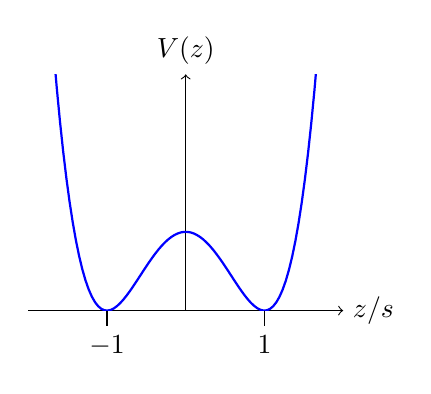
\begin{tikzpicture}
\draw[->](-2,0) -- (2,0)node[right]{$z/s$};
\draw[->](0,0) -- (0,3)node[above]{$V(z)$};
\begin{scope}
\clip (-2,0) rectangle (2,3);
\draw[domain=-2:2,samples=100,blue,thick] plot({\x},{\x*\x*\x*\x - 2*\x*\x + 1});
\end{scope}
\draw(-1,0) -- (-1,-.2)node[below]{$-1$};
\draw(1,0) -- (1,-.2)node[below]{$1$};
\end{tikzpicture}
\end{marginfigure}
\end{exercise}




%---------------------------------------
\chapter{ElMaW Harmonic Oscillator Model}

\begin{marginfigure}
\centering
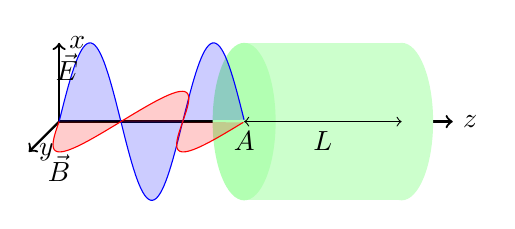
\begin{tikzpicture}[scale=1]
\draw[->,thick] (0,0,0) -- (5,0,0) node[right]{$z$};
\draw[->,thick] (0,0,0) -- (0,1,0) node[right]{$x$};
\draw[->,thick] (0,0,0) -- (0,0,1) node[right]{$y$};

\begin{scope}[shift={(2.35,0,0)}]
\fill[green!20] (0,-1,0) rectangle +(2,2);
\fill[green!30] (0,0,0) ellipse (.4 and 1) node[below,black]{$A$};
\begin{scope}[shift={(2,0,0)}]
\fill[green!20] (0,0,0) ellipse (.4 and 1);
\end{scope}
\end{scope}
\draw[<->] (2.35,0,0) -- (4.35,0,0)node[midway,below]{$L$};
\draw[color=blue,domain=0:2.35,fill=blue,samples=100, fill opacity=0.2] plot (\x,{sin(720/3.14*\x)},0) node[midway,above,black,fill opacity=1,shift={(.1,.4,0)}] {$\vec{E}$};
\draw[color=red,domain=0:2.35,fill=red,samples=100, fill opacity=0.2] plot (\x,0,{sin(720/3.14*\x)}) node[midway,below,black,fill opacity=1,shift={(0,-.3,0)}] {$\vec{B}$};

\end{tikzpicture}
\end{marginfigure}
Early on in Section \ref{sec:elmaw1} we modeled electromagnetic waves as coupled oscillating electric and magnetic fields. The energy density of the electromagnetic wave (energy per unit volume) is 
\beq
u = \frac{1}{2}\left(\epsilon_0 E^2 + \frac{1}{\mu_0}B^2\right).
\eeq
So the total energy of the entire wave in a volume $V$ is found by integrating this over the volume. Because the wave is propagating at speed $c$, we will look at a volume that is a cylinder of cross-sectional area $A$ and length $L$. The total energy of the electric field in this volume is then\arnote{Do the integral on your own.}%
\beq
U_\rmt{electric} = \frac{1}{2}\epsilon_0 A\int\displaylimits_0^L E_0^2\sin^2kz\sin^2\omega t dz = \frac{\epsilon_0}{4}V E_0^2 \sin^2\omega t.
\eeq
The total energy in both the electric and magnetic fields is then
\beq
U = \frac{V}{4}\left( \epsilon_0E_0^2 \sin^2\omega t + \frac{B_0^2}{\mu_0} \cos^2\omega t\right).
\eeq
This looks very similar to a harmonic oscillator which leads us to develop a quantum harmonic oscillator model for the ElMaW.

\section{ElMaW QHO Model}

If we model the electric and magnetic field amplitudes as operators, we could model this energy as a Hamiltonian and use the tools we developed in Chapter \ref{ch:numberbasis}. The operator version of the ElMaW Hamiltonian then looks like this:\marginnote{The ${}+1/2$ factor comes from the details of how we actually do the quantization and make the operators work.}
\beq
\hat{H}_\rmt{ElMaW} = \left(\EAp\EAm + \frac{1}{2}\right)\hbar \omega.
\eeq
\begin{exercise}
What are the raising and lowering operators $\EApm$ in terms of the electric and magnetic field operators $\hat{E}_0$ and $\hat{B}_0$? Note that, since $E_0$ and $B_0$ are both constants, they commute and the factor of $1/2$ is missing.
\end{exercise}

As with the quantum harmonic oscillator, we are now modeling the ElMaW using a number state called a {\em Fock state}. $\ket{n}$ where $n=0,1,2,\ldots$. The Fock states represent individual quanta of energy of an ElMaW with a specific frequency and moving in a specific direction.\marginnote{I've not used the word {\em photon} at all up till now. It is a very misleading word and doesn't clearly convey what is happening. However, most people would call these quanta ``photons''.} The raising and lowering operators $\EApm$ now model the addition and subtraction of energy quanta from the ElMaW. The existence of a ground state $\ket{n}= \ket{0}$ is modeling a vacuum state- the state of the electromagnetic field with no wave propagating. This model has a vacuum energy -- even if $n=0$, there is still an energy eigenvalue of the Hamiltonian: $E_0 = 1/2 \hbar\omega$. This model predicts that the vacuum has an energy associated with it and experiments have shown this to be the case.

We also connect this model to our classical ElMaW model through the intensity of the ElMaW. We define the number operator so that the Fock states are eigenstates of this operator:
\beq
\EN\ket{n} = n\ket{n}.
\eeq
The intensity of the ElMaW is then measured as the rate of change of the average of the number operator in the Fock state basis because the total energy of the ElMaW is measured as $E_n = (n+1/2)\hbar\omega$. So the intensity is the rate of change of the energy per unit area $A$:
\beq
I =\frac{1}{A}\frac{dE}{dt} = \frac{\hbar\omega}{A} \frac{d}{dt}\bra{n}\EN\ket{n} =\frac{\hbar\omega}{A} \frac{dn}{dt}.
\eeq


\section{Fock State Beamsplitter}

We return now to the model we developed in Section \ref{sec:EMbeamsplitter} and now model this situation using our quantized ElMaW model. 

\begin{marginfigure}
\centering
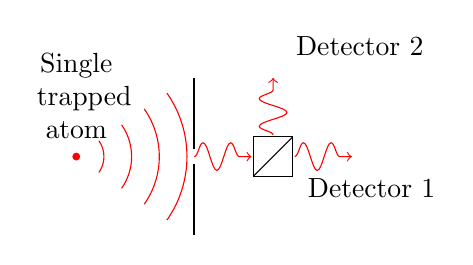
\begin{tikzpicture}[scale=0.5]
\draw (-0.5,-.5) rectangle +(1,1);
\draw (-.5,-.5) -- (.5,.5);
\draw[red,->,decorate, decoration={snake,amplitude=5,segment length=10, post length=.1cm}](-2,0)--(-.55,0) node[midway, above,shift=({0,.2cm})]{};
\draw[red,->,decorate, decoration={snake,amplitude=5,segment length=10, post length=.1cm}](.55,0)--(2,0);
\detector{1}{2.1}{0}{0}
\node at (2.5,-.8) {Detector 1};
\draw[red,->,decorate, decoration={snake,amplitude=5,segment length=10, post length=.1cm}](0,.55)--(0,2);
\detector{1}{0}{2.1}{90}
\node at (2.2,2.8) {Detector 2};
\fill[red] (-5,0) circle(0.1) node[above,black,text width=1cm,align=center,shift={(0,.1cm)}]{Single trapped atom};
\draw[red,decorate,decoration={expanding waves,angle=35}](-5,0) -- (-2,0);
\draw[thick] (-2,.2) -- (-2,2);
\draw[thick] (-2,-.2) -- (-2,-2);
\end{tikzpicture}
\end{marginfigure}

We model the emission of an ElMaW from the single trapped atom as the raising operator into a specific mode so that the atom's emission is modeled by the operator
\beq
\EAp \ket{n} = \sqrt{n+1}\ket{n+1}.
\eeq
If we model the initial Fock state as the vacuum state, then after the atom emits an ElMaW, the quantum state is then $\ket{1}$. We now model the beamsplitter in this basis.%
\begin{marginfigure}\centering
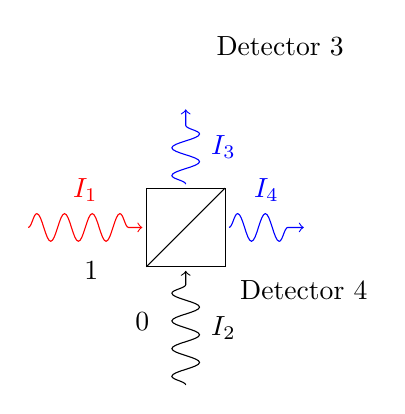
\begin{tikzpicture}
\draw (-0.5,-.5) rectangle +(1,1);
\draw (-.5,-.5) -- (.5,.5);
\draw[->,red,decorate, decoration={snake,amplitude=5,segment length=10, post length=.1cm}](-2,0)--(-.55,0) node[midway, above,shift=({0,.2cm})]{$I_1$};
\node at (-1.2,-.55){$\ket{1}$};
\draw[->,decorate, decoration={snake,amplitude=5,segment length=10, post length=.1cm}](0,-2)--(0,-.55) node[midway, right,shift=({.2cm,0})]{$I_2$};
\node at (-.55,-1.2){$\ket{0}$};
\draw[->,blue,decorate, decoration={snake,amplitude=5,segment length=10, post length=.1cm}](.55,0)--(1.5,0) node[midway, above,shift=({0,.2cm})]{$I_4$};
\draw[->,blue,decorate, decoration={snake,amplitude=5,segment length=10, post length=.1cm}](0,.55)--(0,1.5) node[midway, right,shift=({.2cm,0})]{$I_3$};
\detector{1}{0}{1.6}{90}
\node at (1.2,2.3) {Detector $3$};
\detector{1}{1.6}{0}{0}
\node at (1.5,-.8) {Detector $4$};
\end{tikzpicture}
\end{marginfigure}%
We model the beamsplitter as having two inputs ($1$ and $2$) and two outputs ($3$ and $4$). The beamsplitter itself is modeled as a pair of raising and lowering operators:
\beq
\begin{split}
\EAp^3 =& \frac{1}{\stwo}\left(\EAp^1 - \EAp^2\right)\\
\EAp^4 =& \frac{1}{\stwo}\left(\EAp^1 + \EAp^2\right).
\end{split}
\label{eq:bsraising}
\eeq
\begin{example}
If the input to a beamsplitter is the product state of $\ket{0}$ on input $1$ and $\ket{1}$ on input $2$: $\ket{n_\rmt{input}}=\ket{0}\otimes\ket{1}$, what are the average output states at $3$ and $4$?

\model We model the incoming wave as a product of two Fock states. We'll model the beamsplitter as the quantum operator as described in Eq.~(\ref{eq:bsraising}).

\vis The picture is shown above, but with the input and output states reversed.

\sol The average output for port $3$ is $\avg{\EN_3}$. We write this using Eq.~(\ref{eq:bsraising}) in terms of the input raising and lowering operators:
\bas
\avg{\EN_3} = & \bra{n_\rmt{input}}\EAp^3\EAm^3\ket{n_\rmt{input}}\\
=&\bra{n_\rmt{input}}\left(\frac{1}{\stwo}\left(\EAp^1 - \EAp^2\right) \right)\left(\frac{1}{\stwo}\left(\EAm^1 - \EAm^2\right) \right)\ket{n_\rmt{input}}\\
=&\frac{1}{2}\bra{0}\otimes\bra{1}\left(\EAp^1\EAm^1 -\EAp^1\EAm^2 - \EAp^2\EAm^1  + \EAp^2\EAm^2\right)\ket{0}\otimes\ket{1}\\
=&\frac{1}{2}
\eas\arnote[-1.5cm]{Finish up the missing steps in your notes.}

Similarly, the average output at $4$ is:
\beq
\avg{\EN_4} = \frac{1}{2}.
\eeq

\assess Both of these are what we expect them to be- half the time the ElMaW will be measured at detector $3$ and half the time at detector $4$.

\end{example}

\begin{exercise}
Show that, if the input to the beamsplitter is modeled by an arbitrary Fock state on input $1$ and the vacuum state $\ket{0}$ on input $2$, that the average measurements at the detectors will both be half of the input number.
\end{exercise}



\section{Anti-coincidence}

We are ready to model the anti-coincidence measurement we saw in Section \ref{sec:coincid}. We found experimentally that we never measured the simultaneous arrival of an ElMaW emitted by a single atom at the two output detectors from the beamsplitter. We now modify the definition of the second-order correlation, Eq.~(\ref{eq:gtwo}), so that we can use our Fock state model of the ElMaW. We saw that 
\beq
g^{(2)} = \frac{\avg{I_3(t) I_4(t)}}{\avg{I_3(t)}\avg{I_4(t)}}.
\eeq
We now model the total number of quanta that arrived at the detectors during a time interval $T$ as $n_3$ and $n_4$ for detectors $3$ and $4$. The intensity $I_3$ is then
\beq
I_3 = \frac{\hbar\omega}{A} \frac{n_3}{T}.
\eeq
We will model all of the incoming ElMaWs as having the same frequency and as covering the same area on the detector. This means that the second-order correlation can be written as
\beq
g^{(2)} = \frac{\avg{n_3 n_4}}{\avg{n_3}\avg{n_4}}.
\eeq\arnote{Fill in the missing steps.}
We now model this as the averages of the quantum operators, noting that the number operator is written as the raising and lowering operators:
\beq
g^{(2)} = \frac{\avg{\EAp^3\EAm^3\EAp^4\EAm^4}}{\avg{\EAp^3\EAm^3}\avg{\EAp^4\EAm^4}}.
\label{eq:gtwoquantum}
\eeq
We use this quantum beamsplitter model to calculate the second-order correlation for any input Fock state.

\begin{example}
What is the second-order correlation for the input product state on input ports $1$ and $2$ of a beamsplitter, $\ket{n_\rmt{input}}=\ket{n_1}\otimes\ket{0}$?

\model We again model the beamsplitter as the combined quantum operator with second-order correlation given by Eq.~(\ref{eq:gtwoquantum}).

\vis Our picture hasn't changed.

\sol We know the two values in the denominator from our previous exercise:
\beq
\avg{\EN_3} = \avg{\EN_4} = \frac{n_1}{2} \rmt{ so } \avg{\EN_3}\avg{\EN_4} = \frac{n_1^2}{4}.  
\eeq

We now need the numerator:
\bas
\avg{\EAp^3\EAm^3\EAp^4\EAm^4} =& \frac{1}{4}\bra{n_1}\otimes\bra{0}\left(\EAp^1 - \EAp^2\right) \left(\EAm^1 - \EAm^2\right)\\
{}&\left(\EAp^1 + \EAp^2\right)\left(\EAm^1 + \EAm^2\right) \ket{n_1}\otimes\ket{0}.
\eas
Because of the vacuum state on the right, any term with $\EAm^2$ on the right will be zero. Similarly, any term with $\EAp^2$ on the left will be zero. \arnote{Work this out in your notes.} That leaves just one term that is non-zero:
\bas
\avg{\EAp^3\EAp^4\EAm^3\EAm^4} =& \frac{1}{4}\bra{n_1}\otimes\bra{0}\left( \EAp^1\EAp^1\EAm^1\EAm^1\right)\ket{n_1}\otimes\ket{0} \\
=& \frac{n_1(n_1 - 1)}{4}.
\eas

So the second-order correlation is:
\beq
g^{(2)} = \frac{n_1(n_1 - 1)}{n_1^2}.
\eeq

\assess If we have the case where $n_1 = 1$ then $g^{(2)}\rightarrow 0$ which is what we expect should happen. If there is only a single incoming quanta, we should never measure it at both detectors.


\end{example}

\begin{exercise}
What is the second-order correlation for the input product state on input ports $1$ and $2$ of a beamsplitter, $\ket{n_\rmt{input}}=\ket{1}\otimes\ket{1}$?

\end{exercise}

\begin{exercise}
We introduced the idea of a coherent state model for the quantum harmonic oscillator in Exercise \ref{ex:coherentstate}. Use the model we built in that exercise to show that, for an input coherent state on one arm of the beamsplitter and vacuum on the other arm, $g^{(2)}=1$, which corresponds to what we would expect for a classical coherent wave.
\end{exercise}


%---------------------------------------
\chapter{Part \ref{part4} Review and Test}

This Part started with building a model of angular momentum. We went on to treat central potentials and the hydrogen atom with several perturbations. We then moved to a handful of other topics in quantum mechanics and ended back where we started in looking at quantized ElMaWs.

It is important to practice using these tools to model experiments. The following set of exercises is a good way to test your understanding of these models. Try to do these without referring to the previous text. If you can do all of them and your solutions agree with those provided on the following pages, then you are in pretty good shape to move forward with the material. If not, you should specifically review the material  you do not have mastery of yet, then retry the test exercises.

\begin{exercise}
The electron in a hydrogen atom is placed into a superposition state at $t=0$ of
\beq
\Psi(r,\theta,\phi) = \sqrt{\frac{1}{10}}\psi_{100}(r,\theta,\phi) + \frac{3}{\sqrt{10}}\psi_{321}(r,\theta,\phi)
\eeq
where $\psi_{nlm_l}$ are the eigenstates of the Coulomb interaction model. What is the average distance, with uncertainty, of the electron from the proton?

\end{exercise}

\begin{exercise}
The electron in a hydrogen atom is placed into a superposition state at $t=0$ of
\beq
\Psi(r,\theta,\phi) = \sqrt{\frac{2}{3}}\psi_{200}(r,\theta,\phi) + \sqrt{\frac{1}{3}}\psi_{311}(r,\theta,\phi)
\eeq
where $\psi_{nlm_l}$ are the eigenstates of the Coulomb interaction model. 
\begin{enumerate}
\item What are the possible outcomes if we measure the total angular  momentum of this state? 
\item What are the possible outcomes if we measure the $z$-component of the angular momentum of this state?
\item What are the probabilitites of each of these outcomes?
\item What would the state be after measuring each of these outcomes?
\end{enumerate}
\end{exercise}

\begin{exercise}
Find the lowest energy for an electron confined to a one-dimensional Lennard-Jones potential
\beq
V(x) = \frac{\hbar^2 \varepsilon_0}{2 m x_m^2}\left(\left(\frac{x_m}{x}\right)^{12} -\left(\frac{x_m}{x}\right)^6  \right)
\eeq
for a value of $\varepsilon_0=40$ and over the range of $0.2 \leq x/x_m\leq 4$.
\end{exercise}

\begin{exercise}
The electron in a hydrogen atom is placed into a superposition state at $t=0$ of
\beq
\Psi(r,\theta,\phi) = \sqrt{\frac{2}{5}}\psi_{100}(r,\theta,\phi) - \sqrt{\frac{3}{5}}\psi_{410}(r,\theta,\phi)
\eeq
where $\psi_{nlm_l}$ are the eigenstates of the Coulomb interaction model. 
\begin{enumerate}
\item What would we expect if we measured the average energy of this state?
\item What would we expect for the uncertainty of this measurement?
\item Write down the wavefunction as a function of time after $t=0$, assuming that we haven't measured the state yet.
\end{enumerate}
\end{exercise}

Stop here and don't continue reading until you have completed the exercises.
\newpage
\begin{example}
The electron in a hydrogen atom is placed into a superposition state at $t=0$ of
\beq
\Psi(r,\theta,\phi) = \sqrt{\frac{1}{10}}\psi_{100}(r,\theta,\phi) + \frac{3}{\sqrt{10}}\psi_{321}(r,\theta,\phi).
\eeq
What is the average distance, with uncertainty, of the electron from the proton?

\model We'll use the Coulomb interaction model where $\psi_{nlm_l}$ are the eigenstates of the Hamiltonian.  We can write these in terms of the radial wavefunctions and spherical harmonics and then use our \CAS to do the integration.

\vis The wavefunctions were shown earlier. The visualization doesn't really help here.

\sol The integral we need is similar to Eq.~(\ref{eq:matrixintegral2}):
\beq
\avg{r} = \int\displaylimits_0^\infty r^2 dr\int\displaylimits_0^\pi \sin\theta d\theta \int\displaylimits_0^{2\pi}d\phi\;\Psi^*(r,\theta,\phi) \; r \; \Psi^{}(r,\theta,\phi),
\eeq
where we plug in the superposition state for $\Psi(r,\theta,\phi)$. We use our \CAS to do the integration and get
\beq
\avg{r} = \frac{48 a_0}{5} \approx 9.6 a_0.
\eeq
We also need $\avg{r^2}$ to find the uncertainty. It is very similar:
\beq
\avg{r} = \int\displaylimits_0^\infty r^2 dr\int\displaylimits_0^\pi \sin\theta d\theta \int\displaylimits_0^{2\pi}d\phi\;\Psi^*(r,\theta,\phi) \; r^2 \; \Psi^{}(r,\theta,\phi),
\eeq
which gives $\avg{r^2} = 113.7 a_0^2$. The uncertainty is then
\beq
\Delta r = \sqrt{\avg{r^2}- \avg{r}^2} \approx 4.64 a_0.
\eeq

\assess We got a fairly large average radius with a pretty big spread. Given that the state is mostly in $\psi_{321}$, this makes sense because that state has an average radius of $10.5 a_0$.


\end{example}

\begin{example}
The electron in a hydrogen atom is placed into a superposition state at $t=0$ of
\beq
\Psi(r,\theta,\phi) = \sqrt{\frac{2}{3}}\psi_{200}(r,\theta,\phi) + \sqrt{\frac{1}{3}}\psi_{311}(r,\theta,\phi)
\eeq
where $\psi_{nlm_l}$ are the eigenstates of the Coulomb interaction model. 
\begin{enumerate}
\item What are the possible outcomes if we measure the total angular  momentum of this state? 
\item What are the possible outcomes if we measure the $z$-component of the angular momentum of this state?
\item What are the probabilities of each of these outcomes?
\item What would the state be after measuring each of these outcomes?
\end{enumerate}

\model We use the same model, but this time we measure the angular momentum.

\vis Not much to visualize.

\sol We know that $\hat{L}^2 \ket{nlm_l} = \hbar^2 l(l+1) \ket{nlm_l}$ and $\hat{L}_z \ket{nlm_l} = \hbar m_l \ket{nlm_l}$. So we use the probability tool to get the two probabilities:

\begin{enumerate}
\item The two outcomes are for $l=0$ which gives a measurement of $0$ and for $l=1$ which gives a measurement of $2\hbar^2$.

\item The two outcomes are for $m_l =0$ which gives a measurement of $0$ and for $m_l=1$ which gives a measurement of $\hbar$.

\item The probability of making the two different measurements are
\bas
P(0 \rmt{ or } 0) =& \frac{2}{3}\\
P(2\hbar^2 \rmt{ or } \hbar) = & \frac{1}{3}.
\eas

\item After measuring the first possibility, the state will be represented by the wavefunction $\psi_{200}(r,\theta,\phi)$. The second outcome will result in $\psi_{311}(r,\theta,\phi)$.

\assess The probabilities add up to one.

\end{enumerate}

\end{example}

\begin{example}
Find the lowest energy for an electron confined to a one-dimensional Lennard-Jones potential
\beq
V(x) = \frac{\hbar^2 \varepsilon_0}{2 m x_m^2}\left(\left(\frac{x_m}{x}\right)^{12} -\left(\frac{x_m}{x}\right)^6  \right)
\eeq
for a value of $\varepsilon_0=40$ and over the range of $0.2 \leq x/x_m\leq 4$.

\model We are going to use a numerical model to solve this. Although a quick search on the internet indicates there may be exact solutions, it will be easier to get the lowest energy by trying a numerical model.

\vis The potential is shown in Fig.~\ref{fig:LJP}
\begin{marginfigure}




\centering
\begin{tikzpicture}
\draw[->](0,0) -- (3,0)node[right]{$x/x_m$};
\draw[->](0,-2) -- (0,1)node[above]{$V(z)$};
\begin{scope}
\clip (0,-2) rectangle (3,1);

\begin{sagesilent}
x=var('x')
t = var('t')
x_coords = [t for t in srange(.95,3.0,.05)]
y_coords = [8/(t**12)-8/(t**6) for t in srange(.95,3.0,.05)]
output = ""
for i in range(0,len(x_coords)-1):
    output += r"\draw[blue, thick] (%f cm ,%f cm)--(%f cm ,%f cm);"%(x_coords[i],y_coords[i],x_coords[i+1],y_coords[i+1])
\end{sagesilent}

\sagestr{output}


\end{scope}
\draw(1,0) -- (1,-.2)node[below]{$1$};
\draw(2,0) -- (2,-.2)node[below]{$2$};
\end{tikzpicture}
\caption{ }
\label{fig:LJP}
\end{marginfigure}

\end{example}

\sol We first need to write the TISWE in dimensionless parameters. It makes sense to use $\xi = x/x_m$ as the dimension. We multiply through by $2m x_m^2 /\hbar^2$ and then call our energy parameter
\beq
\varepsilon = \frac{-2 m x_m^2 E}{\hbar^2}.
\eeq
This gives us a dimensionless TISWE of
\beq
\frac{d^2\psi}{d\xi^2} - \left(\varepsilon + \varepsilon_0\left(\frac{1}{\xi^{12}} - \frac{1}{\xi^6} \right)\right).
\eeq
Because we know we want our wavefunction to go to zero at $\xi = 4$, we will use that as the known starting point for our shooting method. We'll set $\psi(4)=0$ and $\psi'(4)=0.001$ in the numerical solver. We use the \CAS techniques described earlier and find a dimensionless energy eigenvalue of
\beq
\varepsilon \approx 0.4363915\ldots
\eeq

\assess When plotting the eigenfunction corresponding to this energy, we find that it still isn't quite right at the left boundary of $\xi=0.2$. This is a hard potential to solve, but this gets us close.

\begin{example}
The electron in a hydrogen atom is placed into a superposition state at $t=0$ of
\beq
\Psi(r,\theta,\phi) = \sqrt{\frac{2}{5}}\psi_{100}(r,\theta,\phi) - \sqrt{\frac{3}{5}}\psi_{410}(r,\theta,\phi).
\eeq
\begin{enumerate}
\item What would we expect if we measured the average energy of this state?
\item What would we expect for the uncertainty of this measurement?
\item Write down the wavefunction as a function of time after $t=0$, assuming that we haven't measured the state yet.
\end{enumerate}

\model We'll model the eigenfunctions of the energy operator as the $\psi_{nlm_l}$. As we found earlier, the energies are then 
\beq
E_n = -\frac{E_1}{n^2}.
\eeq

\vis Not much to see here.

\sol 
\begin{enumerate}
\item The average energy is just the average of the Hamiltonian. Since the $E_n$ values are the eigenvalues, we get
\beq
\avg{E} = \frac{2}{5} \left(\frac{-E_1}{1^2}\right) + \frac{3}{5} \left(\frac{-E_1}{4^2}\right) = -\frac{7}{16}E_1.
\eeq

\item We also need $\avg{E^2}$ to find the uncertainty. Since the $E_n$ are eigenvalues, this is straight-forward:
\beq
\avg{E^2} = \frac{2}{5} \left(\frac{-E_1}{1^2}\right)^2 + \frac{3}{5} \left(\frac{-E_1}{4^2}\right)^2 = \frac{103}{253}E_1^2. 
\eeq
The uncertainty in the energy measurement is then
\beq
\Delta E = \sqrt{\avg{E^2} - \avg{E}^2} = \frac{3\sqrt{3}}{8\sqrt{2}}E_1.
\eeq

\item We know the eigenenergies of both pieces of the wavefunction. So the time evolution of this state is just
\beq
\Psi(r,\theta,\phi,t) = \sqrt{\frac{2}{5}}\E{-\I E_1 t/\hbar}\psi_{100}(r,\theta,\phi) - \sqrt{\frac{3}{5}}\E{-\I E_1 t/(16 \hbar)}\psi_{410}(r,\theta,\phi).
\eeq

\assess The energy is reasonable-- slightly more than ${-E_1}$, which is what we would expect for a state made up of $n=1$ and $n=4$ pieces.

\end{enumerate}

\end{example}



%sagemathcloud={"latex_command":""}